\graphicspath{{./chapters/chapter4/}}

\def\c{cr}
\def\hc{\hat{cr}}
\def\d{\Lambda}
\def\ind{\mathbbm{1}}
\def\oc{Online\_Cluster}
\def\mem{\mathcal M}
\def\E{\mathbb{E}}
\def\R{\mathbb{R}}
\def\O{\mathcal{O}}
\def\calP{\mathcal{P}}
\def\dc{Data\_Copy\_Detect}
\def\a{\kappa}
\def\hq{\widehat{q(B(x, r))}}
\def\alpaca{\epsilon}




\chapter{Appendix for Chapter 5}

\section{An Example over the Halfmoons dataset}\label{sec:app_experiments}

In this section, we give an overview of our experiments over the Halfmoons dataset. Further details can be found in sec


\begin{figure}[ht]
	\begin{subfigure}{0.45\textwidth}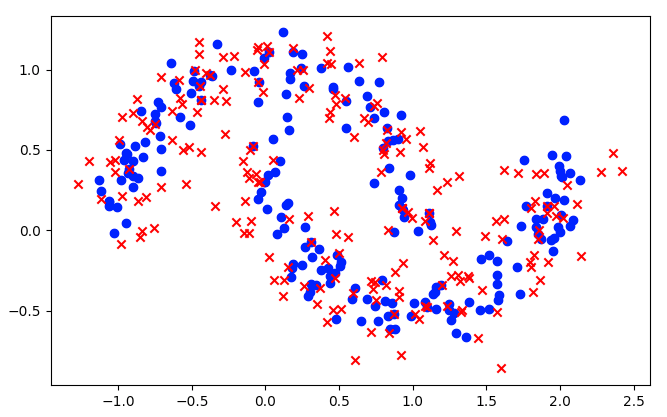
\includegraphics[width=\linewidth]{rho1.png}\caption{$\rho = 0.1$}
	\end{subfigure}\hspace*{\fill}
	\begin{subfigure}{0.45\textwidth}
	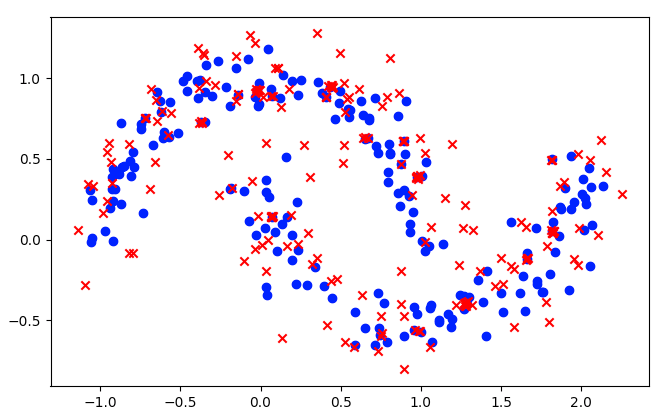
\includegraphics[width=\linewidth]{rho4.png}\caption{$\rho = 0.4$}
	\end{subfigure}
	\caption{The blue points are sampled from $p$, and the red points from $q$. The parameter $\rho$ is the proportion of examples of $q$ that are from $q_{copy}$, with the rest coming from $q_{underfit}$. The combination of $q_{copy}$ and $q_{underfit}$ make data-copying detection difficult for \cite{MCD2020}'s method.}
	
	\label{fig:halfmoons}
\end{figure}

Our theoretical results show that given enough data, Algorithm \ref{alg:main} is guaranteed to detect data-copying. By contrast, the non-parametric test provided in \cite{MCD2020} can only guarantee detection in cases in which data-copying \textit{globally} occurs. For more local instances of data-copying, they rely on $k$-means clustering to partition the input space into localized regions, and then run their global test over each region separately.

Their approach clearly cannot detect all forms of data-copying -- a pathological generative distribution might copy in complex regions that are impossible to find using $k$-means clustering. However, for many practical examples considered in their paper, \cite{MCD2020} demonstrated considerable success with this approach. 

This motivates the following question: 
\begin{quote}
Do there exist natural data distributions over which Algorithm \ref{alg:main} offers a meaningful advantage?
\end{quote} 

We provide a partial answer to this question by experimentally comparing our approach with \cite{MCD2020}'s over a simple example on the half moons dataset.

\subsection{Experimental Setup}

\paragraph{Data Distribution:} Our data distribution, $p$, is the Halfmoon dataset with Gaussian noise ($\sigma = 0.1$).  

\paragraph{Generated Distribution:} Our generated distribution, $q$, is trained from an i.i.d sample of 2000 points from $p$, $S \sim p^{2000}$. Because our focus is on distinguishing \textit{data-copy detection} algorithms, we design $q$ to have a large amount of data-copying that is nevertheless subtle to detect. The key idea is to let $q$ be a mixture of two distributions, $q_{copy}$ and $q_{underfit}$. $q_{copy}$ will be an egregious data copier, and $q_{underfit}$ will be designed to average away the effects of $q_{copy}$. 

To construct $q_{copy}$, we first select a subset, $S' \subset S$, of $20$ training examples. Then, we define $q_{copy}$ to randomly output points from $S'$ combined with a small amount of spherical noise (with radius $0.02$). Thus, $q_{copy}$ can be sampled from by sampling a point, $x$, from $S'$ at uniform, and returning $x+\eta$ where $\eta$ is drawn at uniform from a disk of radius $0.02$.

To construct $q_{underfit}$, we combine our original data distribution, $p$, with a moderate amount of spherical noise (with radius $0.25$). Thus, $q_{underfit}$ can be sampled from by first sampling $x \sim p$, and returning $x+ \eta$ where $\eta$ is drawn at uniform from a disk of radius $0.25$. This distribution is meant to represent a fairly noisy and thus underfit version of $p$. 

Finally, we define $q$ as a mixture of $q_{copy}$ and $q_{underfit}$, with $q$ outputting a point from $q_{copy}$ with probability $\rho$. In total, we have $$q = \rho \cdot q_{copy} + (1-\rho) \cdot q_{good}.$$ We let, $\rho$, the weight of $q_{copy}$ within the mixture, be a varying parameter that gives rise to different generated distributions. Intuitively, the larger $\rho$ is, the higher the data-copying rate. This is illustrated in Figure \ref{fig:halfmoons}. In the both panels, we plot a sample of $200$ training points $p$ along with $200$ points from $q$. In the left panel, we let $\rho = 0.1$ in the right, we use $\rho = 0.4$. Although both cases show examples of data-copying, the right panel shows a visibly higher level of it. This is expected, as it is drawn from a distribution in which $q_{copy}$ is much more likely to be queried. 

\paragraph{Data-copying Detection Algorithms:} We run our algorithm, \dc{}, on $(S, q)$, We fix $\lambda = 20$ and $\gamma = 0.00025$ as constants for data-copy detection. $\lambda$ represents a healthy level of data-copying, and $\gamma = 0.00025$ ensures that our condition for 'copying' is quite stringent. Full details of our implementation (including our practical choices for parameters such as $b$ and $m$) are given in Appendix \ref{sec:experiments}.

For comparison, we also include an implementation of \cite{MCD2020}'s algorithm with varying amounts of clusters being used for the initial $k$-means clustering. To avoid confusion with the intrinsic dimension, $k$, we let $c$ denote the number of clusters, and consider $c \in \{1, 5, 10, 20\}$.

\subsection{Results}

The results are summarized in Table \ref{results}, with each column corresponding to a given choice of $p, q$ (determined by the parameter $\rho$), and each row corresponding to a separate data-copying detection algorithm. As a baseline, we include the case where $q = p$ (meaning we have a perfect generated distribution) in the first column.

We run our algorithm with parameters $\lambda$ and $\gamma$ fixed as $20$ and $0.00025$ in all cases. For \cite{MCD2020}'s algorithm, we consider their data-copy detection score over the most egregious cluster. 

Although our algorithm outputs real number estimates of the true data-copying rate, $\c_q$, \cite{MCD2020}'s algorithm outputs a score indicating the statistical significance of their metric under a null hypothesis of no data-copying occurring. To facilitate a simple comparison between our methods, for all algorithms, we simply output a simple yes or no to indicate whether our results were statistically significant up to the $p=0.05$ level. We include full results of our experiments along with several extensions (with varying parameters) in section \ref{sec:experiments_details}.

As expected, neither of our algorithms detect data-copying on the baseline, $q = p$. However, in all other cases, our algorithm successfully detects data-copying. On the other hand, for the smaller values of $\rho$, \cite{MCD2020}'s does not. Their algorithm is only able to achieve detection when the weight of $\rho = 0.4$, and even in this case they are unable to consistently do so.  

These results match the simple intuition of our algorithms. As seen in Figure \ref{fig:halfmoons}, the red data is sometimes very close to the blue data (when it comes from $q_{copy}$) but at other times fairly distant (when it comes from $q_{underfit}$). These effects have a strong canceling effect in \cite{MCD2020}'s test. However, our test is able to adjust for this by considering each training example separately. 


\begin{table}[h]
\caption{Statistical Significance of data-copying Rates over Halfmoons} \label{results}
\begin{center}
\begin{tabular}{ |c||c|c|c|c|c| } 
 \hline
 \textbf{Algo} & $\mathbf{q = p}$ & $\mathbf{\rho = 0.1}$ & $\mathbf{0.2}$ & $\mathbf{0.3}$ & $\mathbf{0.4}$ \\ 
 \hline
 \hline
 \textbf{Ours} & \color{blue}no & \color{red}yes & \color{red}yes & \color{red}yes & \color{red}yes \\ 
 \hline
 $\mathbf{c=1}$ & \color{blue}no & \color{blue}no & \color{blue}no & \color{blue}no & \color{blue}no \\ 
 \hline
 $\mathbf{c=5}$ & \color{blue}no & \color{blue}no & \color{blue}no & \color{blue}no & \color{red}yes \\ 
 \hline
 $\mathbf{c=10}$ & \color{blue}no & \color{blue}no & \color{blue}no & \color{blue}no & \color{red}yes \\ 
 \hline
 $\mathbf{c=20}$ & \color{blue}no & \color{blue}no& \color{blue}no & \color{red}yes & \color{red}yes\\ 
 \hline
\end{tabular}
\end{center}
\end{table}

 \subsection{Further Experimental Details}\label{sec:experiments_details}

We begin by reviewing the definitions of $p$ and $q$. $p$ is the Halfmoons dataset with Gaussian noise $(\sigma = 0.1)$. To define $q$, we have a mixture of two distributions, $q_{copy}$ and $q_{underfit}$, which are defined as follows.

We draw $S \sim p^{2000}$ i.i.d, and then randomly select $S' \subset S$ with $|S'| = 20$. These points will form a basis for the support of $q_{copy}$. To sample $x \sim q_{copy}$, we take the following two steps.
\begin{enumerate}
	\item Sample $z \sim S'$ at uniform.
	\item Sample $\eta \sim U(B(0, 0.02))$, where $U(B(0, r))$ denotes the uniform distribution over the ball of radius $r$. 
	\item Output $x = z + \eta$.
\end{enumerate}
$q_{copy}$ can be thought of as an egregious data memorizer that injects a small amount of noise to give its inputs some (paltry) variety. 

By contrast, to sample $x \sim q_{underfit}$, we do the following:
\begin{enumerate}
	\item Sample $z \sim p$.
	\item Sample $\eta \sim U(B(0, 0.25))$.
	\item Output $x = z + \eta$.
\end{enumerate}
In this case, the larger amount of noise serves to induce \textit{underfitting}, in which $q_{copy}$ does not assign the support of $p$ enough probability mass. 

Finally, to sample from $q$, we do the following.
\begin{enumerate}
	\item With probability $\rho$, sample $x \sim q_{copy}$.
	\item With probability $1 - \rho$, sample $x \sim q_{underfit}$. 
\end{enumerate}

\paragraph{\cite{MCD2020}'s test:} Their test works as follows. Let $S$ denote the original training sample, $Q$ denote a sample of generated examples, with $Q \sim q^{n}$, and $P$ denote a fresh set of test examples, with $P \sim p^n$. They then check to see if $Q$ is systematically closer to $S$ than $P$, (thus suggesting data copying). To do so, they use a statistical test as follows:
\begin{enumerate}
	\item Let $S = \{x_1, x_2, \dots, x_n\}$, $P = \{y_1, y_2, \dots, y_n\}$, $Q = \{z_1, z_2, \dots, z_n\}$. 
	\item Let $\Delta$ denote the number of pairs $(i, j)$ for which $d(y_i, S) < d(z_j, S)$. A large value of $\Delta$ indicates that a \textit{small} amount of data copying, as it implies that $Q$ is further from $S$ than $P$. A small value of $\Delta$ indicates a \textbf{large} amount of data copying.
	\item Reflecting this, let $Z = \frac{\Delta - \frac{n^2}{2}}{\sqrt{\frac{n^2(2n+1)}{12}}}$. This gives a $Z$-score of $\Delta$. \cite{MCD2020} show that, $p = q$, then the probability of results as significant as $Z < -5$ would be at most the probability of getting a $-5\sigma$ event when sampling from a Gaussian. We use $Z < -3$ to indicate \textit{statistically significant results}, and output the corresponding $P$-values ($P =  0.0027$ being significant) in our results. 
\end{enumerate}

Finally, to account for data copying occurring within specific regions, \cite{MCD2020} perform a preprocessing step in which they cluster the training data, $S$ into $c$ regions using $k$-means clustering. They then run their test separately on each region by assigning points from $P$ and $Q$ into the regions containing them. We output the \textit{lowest} $Z$-score over any region, and vary the number of clusters with $c= 1, 5, 10, 20$. 

\paragraph{Our test:} We run Algorithm \ref{alg:main} with input $(S, q)$ with a few adjustments.
\begin{enumerate}
	\item We directly set $m = 200,000$. While the theoretical value of $m$ is significantly higher (growing $O(n^2)$), we note that this is primarily done for achieving theoretical guarantees. In practice, often a much lower amount of data is needed.
	\item For $Est(x, r, S)$, we set $b= 400$, which is a bit lower than the theoretically predicted value. As for $m$, we do this because for practical (and well-behaved) datasets, $Est(x, r, S)$ converges much more quickly than theory suggests. 
	\item We set $\lambda = 20$ and $\gamma = \frac{1}{4000}$, giving relatively stringent conditions on data copying. 
\end{enumerate}
Finally, our test outputs, $\hat{\c}_q$, which is an estimate of the data copy rate. Technically, any non-zero of $\hat{\c}_q$ indicates a degree of data copying. To facilitate a more direct comparison with \cite{MCD2020}, we convert our results into statistical tests by doing the following.
\begin{enumerate}
	\item We compute $\hat{\c}_p$, which is an estimate for the data copying rate when the generated distribution exactly equals $p$ over $1000$ different instances (each instance corresponding to a freshly drawn training set $S$).
	\item We then compute $\hat{\c}_q$ when $q$ is as above.
	\item We finally output the fraction of the time that $\hat{\c}_p > \hat{\c}_q$, thus giving us a P-value by giving us the rate at which the null-hypothesis gives results as significant as those that we observe. 
\end{enumerate} 

\paragraph{Results:} We give a more complete version of Table \ref{results}, with the $P$-values themselves being outputted in the table. For consistency, we output the median $P$-value obtained over 10 runs for each experiment. 

\begin{table}[h]
\caption{P-values of data-copying Rates over Halfmoons} \label{results:full}
\begin{center}
\begin{tabular}{ |c||c|c|c|c|c| } 
 \hline
 \textbf{Algo} & $\mathbf{q = p}$ & $\mathbf{\rho = 0.1}$ & $\mathbf{0.2}$ & $\mathbf{0.3}$ & $\mathbf{0.4}$ \\ 
 \hline
 \hline
 \textbf{Ours} & \color{blue}1.000 & \color{red}0.000 & \color{red}0.000 & \color{red}0.000 & \color{red}0.000 \\ 
 \hline
 $\mathbf{c=1}$ & \color{blue}0.5412 & \color{blue}1.000 & \color{blue}1.000 & \color{blue}0.858 & \color{blue}0.026 \\ 
 \hline
 $\mathbf{c=5}$ & \color{blue}0.113 & \color{blue}0.976 & \color{blue}0.780 & \color{blue}0.081 & \color{red}0.007 \\ 
 \hline
 $\mathbf{c=10}$ & \color{blue}0.090 & \color{blue}0.814 & \color{blue}0.294 & \color{blue}0.013 & \color{red}0.000 \\ 
 \hline
 $\mathbf{c=20}$ & \color{blue}0.035 & \color{blue}0.279& \color{blue}0.093 & \color{red}0.005 & \color{red}0.000\\ 
 \hline
\end{tabular}
\end{center}
\end{table}

We also remark that the computed data-copying rates by our algorithm exactly match the value of $\rho$ in all cases (up to 3 decimal points).

\section{Estimating $k$}\label{sec:estimating_alpha}

The main idea of our method is to simply pick any point $x_i$ in the training sample, $S = \{x_1, x_2, \dots, x_n\}$, choose two small balls centered at $x_i$, and then measure the ratio of their probability masses as well as their radii. For sufficiently small balls, these ratios will be related by a power of $k$, and we can consequently just solve for an estimate of $k$, $\hat{k}$. Finally, since for our purposes it is extremely important that our estimate be \textit{exactly} correct, we round $\hat{k}$ to the nearest integer. While this clearly fails in cases that $k$ is not an integer, for most distributions $k$ precisely equals the dimension of the underlying data manifold (see for example Proposition \ref{prop:manifold_works}). These steps are enumerated in the following algorithm, $Estimate\_k(S)$. 

\begin{algorithm}
   \caption{$Estimate\_k(S)$}
   \label{alg:estimate_alpha}

   \DontPrintSemicolon

	$n \leftarrow |S|$\;
	
	Pick $x \in S$ arbitrarily.\;
	
   $b \leftarrow \frac{64(d+2)\ln\frac{16n}{\delta}}{\epsilon^2}.$\;
   
   $r_* = \min \{r: |S \cap B(x, r)| = 2b\}$.\;
   
  $s_* =\min \{s: |S \cap B(x, s)| = b\}$\;
  
  $\hat{k} = round \left(\frac{1}{\log_2 \frac{r_*}{s_*}} \right)$\;
  
  Return $\hat{k}$. 

\end{algorithm}

We now give sufficient conditions under which Algorithm \ref{alg:estimate_alpha} successfully recovers $k$. 

\begin{proposition}
Let $p$ be an $k$-regular distribution, and let $\delta > 0$ be arbitrary. Let $\phi = \frac{1}{2k}$. Then there exists a constant $C$ such that if $$n \geq C\frac{d\ln\frac{d}{\delta\phi p_\phi}}{\phi^2 p_\phi},$$ with probability at least $1 - \delta$ over $S \sim p^n$, $Estimate\_k(S) = k$. 
\end{proposition}

\begin{proof}
We begin by first applying standard uniform convergence over $\ell_2$ balls in $\R^d$ (which have a VC dimension of at most $d+2$). To this end, let $$\beta_n = \sqrt{\frac{4(d+2)\ln \frac{16n}{\delta}}{n}}.$$ Then by the standard result of Vapnik and Chervonenkis, with probability $1-\delta$ over $S \sim p^n$, for all $x \in \R^d$ and all $r > 0$, 
\begin{equation}\label{aeqn:VC}
\frac{|S \cap B(x,r)|}{n} - \beta_n\sqrt{\frac{|S \cap B(x,r)|}{n}} \leq p(B(x,r)) \leq \frac{|S \cap B(x,r)|}{n} + \beta_n^2 + \beta_n\sqrt{\frac{|S \cap B(x,r)|}{n}}.
\end{equation}

Next, assume that 
\begin{equation}\label{aeqn:bound_n}
n \geq \frac{1776(d+2)\ln \left(\frac{28416(d+2)}{\delta \phi^2 p_\phi} \right)}{\phi^2 p_\phi}.
\end{equation} 
It is clear that for an appropriate constant, we have $n = O \left(\frac{d\ln\frac{d}{\delta \phi p_\phi}}{\phi^2 p_\phi} \right)$. Thus, it suffices to show that if Equation \ref{aeqn:VC} holds, then $\hat{k} = k$ (as the former holds with probability $1-\delta$ over $S$). We now show the following claim.

\textbf{Claim:} Let $r > 0$ be any radius with $|S \cap B(x, r)| \geq b$. Then $$\left(1 + \frac{\phi}{9}\right)^{-1} \leq \frac{|S \cap B(x, r)|}{n p(B(x, r))} \leq \left(1 + \frac{\phi}{9} \right).$$ 

\begin{proof} From the definition of $b$, we have that \begin{equation}\label{aeqn:defining_b}\frac{b}{n} = \frac{400(d+2)\ln\frac{16n}{\delta}}{n\phi^2} = \frac{100\beta_n^2}{\phi^2}.\end{equation} Let $c = \sqrt{\frac{b'}{n\beta_n^2}}$. Then $b' \geq b$ implies that $c \geq \frac{10}{\phi}$. It follows that \begin{equation}\label{aeqn:c_stuff}\frac{c+1}{c^2} \leq \frac{1}{c-1} \leq \frac{\phi}{9}.\end{equation} Substituting Equations \ref{aeqn:defining_b} and \ref{aeqn:c_stuff} into  Equation \ref{aeqn:VC}, we have 
\begin{equation}\label{aeqn:epsilon_lower_bound}
\begin{split}
\frac{b'}{np(B(x, r))} &\geq \frac{\frac{b'}{n}}{\frac{b'}{n} + \beta_n^2 + \beta_n \sqrt{\frac{k'}{n}}} \\
&= \frac{c^2}{c^2 + 1 + c} \\
&= \left(1 + \frac{c+1}{c^2} \right)^{-1} \\
&\geq \left(1 + \frac{\phi}{9}\right)^{-1}
\end{split}
\end{equation}
and 
\begin{equation}\label{aeqn:epsilon_upper_bound}
\begin{split}
\begin{split}
\frac{b'}{np(B(x, r))} &\leq \frac{\frac{b'}{n}}{\frac{b'}{n} - \beta_n \sqrt{\frac{b'}{n}}} \\
&= \frac{c^2}{c^2 - c} \\
&= 1 + \frac{1}{c-1} \\
&\leq 1 + \frac{\phi}{9},
\end{split}
\end{split}
\end{equation}
Together, Equations \ref{aeqn:epsilon_lower_bound} and \ref{aeqn:epsilon_upper_bound} imply our claim.
\end{proof}

We now return to the proof of Proposition \ref{prop:est_works}. We now show that $$p(B(x, s_*) \leq p(B(x, r_*)) \leq p_\phi.$$ To do so, we first bound $\beta_n^2$ as follows. We have, 
\begin{equation}\label{aeqn:bound_alpha_n}
\begin{split}
\beta_n^2 &= \frac{4(d+2)\ln(16n/\delta)}{n} \\
&= 4(d+2) \ln \left(\frac{28416(d+2)}{\delta \phi^2 p_\phi}\ln\left(\frac{28416(d+2)}{\delta \phi^2 p_\phi} \right)\right) \frac{\phi^2 p_\phi}{1776(d+2)\ln \left(\frac{28416(d+2)}{\delta \phi^2 p_\phi} \right)} \\
&\leq 8(d+2)\ln \left(\frac{28416(d+2)}{\delta \phi^2 p_\phi}\right) \frac{\phi^2 p_\phi}{1776(d+2)\ln \left(\frac{28416(d+2)}{\delta \phi^2 p_\phi} \right)} \\
&= \frac{p_\phi \phi^2}{222}.
\end{split}
\end{equation}
Next, by Equations \ref{aeqn:VC} and \ref{aeqn:bound_alpha_n} along with the fact that $b = \frac{100\beta_n^2}{\phi^2}$ (Equation \ref{aeqn:defining_b}) that 
\begin{equation*}
\begin{split}
p(B(x, r_*)) &\leq \frac{|S \cap B(x, r_*)|}{n} + \beta_n^2 + \beta_n \sqrt{\frac{|S \cap B(x, r_*)|}{n}} \\
&= \frac{2b}{n} + \beta_n^2 + \beta_n\sqrt{\frac{2b}{n}} \\
&= \beta_n^2\left(\frac{200}{\phi^2} +1 + \frac{20}{\phi}\right) \\
&\leq \frac{p_\phi \phi^2}{222}\frac{221}{\phi^2}  = p_\phi.
\end{split}
\end{equation*}
It follows from Definition \ref{def:regular} that 
\begin{equation}\label{aeqn:using_regular}
\left(1 + \frac{\phi}{3}\right)^{-1}\frac{p(B(x, r_*))}{p(B(x, s_*))} \leq \frac{r_*^k}{s_*^k} \leq \left(1 + \frac{\phi}{3}\right)\frac{p(B(x, r_*))}{p(B(x, s_*)}.\end{equation} 

However, $|S \cap B(x, s_*)| = b$ and $|S \cap B(x, r_*)| = 2b$, which means that we can safely apply our claim to both of these cases. By substituting Equations \ref{aeqn:epsilon_lower_bound} and \ref{aeqn:epsilon_upper_bound} (for both $r_*$, $s_*$) into Equation \ref{aeqn:using_regular}, along with the fact that $\left(1+\frac{\phi}{3}\right)\left(1 + \frac{\phi}{9}\right) \leq \left(1 + \frac{\phi}{2}\right)$, it follows that 
\begin{equation}\label{aeqn:bound_ratio}
\left(1 + \frac{\phi}{2}\right)^{-1} \leq \frac{r_*^k}{2s_*^k} \leq \left(1 + \frac{\phi}{2}\right)
\end{equation}

Finally, by taking logs of Equation \ref{aeqn:bound_ratio} and simplifying, we have that 
\begin{equation*}
\frac{k}{1 + \log_2 \left(1 + \frac{\phi}{2}\right)} \leq \frac{1}{\log_2 \frac{r_*}{s_*}} \leq \frac{k}{1 - \log_2 \left(1 + \frac{\phi}{2} \right)}
\end{equation*}
It consequently suffices to show that $k$ is the unique integer between $\frac{k}{1 + \log_2 \left(1 + 8\epsilon\right)}$ and $\frac{k}{1 - \log_2 \left(1 + 2\epsilon\right)}$. However, this is simply a result of the assumption that $\phi = \frac{1}{2k}$ and standard manipulations, which completes the proof. 
\end{proof}

\section{Proofs}

All proofs to theorems and propositions in the main body are in this section. For each result, we include a restatement for convenience. 

\subsection{Proof of Theorem \ref{thm:KDE}}

We prove a stronger version of Theorem \ref{thm:KDE}.

\begin{theorem}[Theorem \ref{thm:KDE}]
Let $1 < \lambda$ and $\gamma > 0$. Let $\sigma_n$ be a sequence of bandwidths and $K$ be any regular kernel function. For any $n > 0$ there exists a probability distribution $\pi$ with full support over $\R^d$ such for any $S \sim \pi^n$, a KDE trained with bandwidth $\sigma_n$ and kernel function $K$ has data-copy rate $\c_q \geq \frac{1}{2}$.
\end{theorem}

We begin by giving necessary conditions for a kernel $K$ to be regular.

\begin{definition}\label{defn:regular_kernel}
A kernel function, $K: \R^d \to \R_{\geq 0}$ is regular if it satisfies the following conditions.
\begin{enumerate}
	\item $K$ is radially symmetric. That is, there exists $h: \R \to \R$ such that $K(x) = h(||x||)$.
	\item $K$ is regularized. That is, $\int_{\R^d} K(x)dx = 1$.
	\item $K$ decays to $0$. That is, $\lim_{t \to \infty} h(t) = \lim_{t \to -\infty}h(t) = 0$. 
\end{enumerate}
\end{definition}

It is well known that under suitable choices of $\sigma_n$ and several technical assumptions that a regular KDE converges towards the true data distribution in the large sample limit. We now prove Theorem \ref{thm:KDE}.

\begin{proof}
Fix any $n$, and for convenience let denote $\sigma_n$ by $\sigma$. Because $K$ is non-negative, by condition 2. of Definition \ref{defn:regular_kernel}, there exists $R > 0$ such that $\int_{||x|| \leq R} K(x)dx = \frac{1}{2}$. Let $$D = R\sigma \left(\max\left(2n\lambda, \frac{1}{\gamma}\right)\omega_d\right)^{1/d},$$ where $\omega_d$ denotes the volume of the unit ball in $d$ dimensions. We let $\pi$ denote the uniform distribution over $[0, D]^d$, and claim that this suffices. 

Let $S \sim \pi^n$ be a training sample, with $S = \{x_1, x_2, \dots, x_n\}$, and let $q$ be a KDE trained from $S$ with bandwidth $\sigma$ and kernel function $K$. Suppose $x \sim q$ satisfies that $x \in B(x_i, R\sigma)$. We claim that $q$ $(\lambda, \gamma)$-copies $x$.

To see this, it suffices to bound $\pi((B(x_i, R\sigma))$ and $q(B(x_i, R\sigma))$. The former quantity satisfies
\begin{equation*}
\begin{split}
\pi((B(x_i, R\sigma)) &\leq \frac{vol(B(x_i, R\sigma))}{D^d} \\
&= \frac{\omega_d(R\sigma)^d}{D^d} \\
&= \frac{1}{\max\left(2n\lambda, \frac{1}{\gamma}\right)} \\ 
&\leq \min\left(\gamma, \frac{1}{2n\lambda}\right),
\end{split}
\end{equation*}
which implies that the third condition of Definition \ref{defn:data_copy} is met. Meanwhile, $q((B(x_i, R\sigma))$ can be bounded as
\begin{equation*}
\begin{split}
q((B(x_i, R\sigma)) &= \int_{B(x_i, R\sigma)} \frac{1}{n\sigma}\sum_{j = 1}^n K \left(\frac{x - x_j}{\sigma} \right)dx \\
&\geq \int_{B(x_i, R\sigma)} \frac{1}{n\sigma}K \left(\frac{x - x_i}{\sigma} \right)dx \\
&= \int_{||u|| \leq R} \frac{1}{n}K(u)du \\
&\geq \frac{1}{2n},
\end{split}
\end{equation*}
which implies that $q((B(x_i, R\sigma)) \geq \lambda p(B(x_i, R\sigma))$ giving the second condition of Definition \ref{defn:data_copy}. Thus, it follows that $q$ $(\lambda,\gamma)$-copies all $x \in B(x_i, R\sigma)$. It consequently suffices to bound $q\left(\bigcup_{i= 1}^n B(x_i, R\sigma)\right)$. 

To do so, let $\eta$ denote the probability distribution over $\R^d$ with probability density function $\eta(x) = \frac{1}{\sigma}K(\frac{x}{\sigma})$, and let $\hat{q}$ denote the probability density function induced by the following random process:
\begin{enumerate}
	\item Select $1 \leq i \leq n$ at uniform.
	\item Select $x \sim \eta$.
	\item Output $x + x_i$.
\end{enumerate}
The key observation is that $\hat{q}$ has precisely the same density function as $q$ -- $q$s density function is clearly a convolution of selecting $x_i$ and then adding $x \sim \eta$. Applying this, we have
\begin{equation*}
\begin{split}
\Pr_{x \sim q}\left[x \in \bigcup_{i= 1}^n B(x_i, R\sigma)\right] &= \Pr_{x \sim \hat{q}}\left[x \in \bigcup_{j= 1}^n B(x_j, R\sigma)\right] \\
&= \frac{1}{n} \sum_{i=1}^n \Pr_{x \sim \tau}\left[x \in \left(\bigcup_{j= 1}^n B(x_j, R\sigma) - x_i\right)\right]\\
&\geq \frac{1}{n} \sum_{i=1}^n \Pr_{x \sim \tau} \left[x \in \left(B(x_i, R\sigma) - x_i\right)\right] \\
&= \int_{B(0, R\sigma)} \tau(x)dx \\
&= \int_{B(0, R\sigma)} \frac{1}{\sigma} K\left(\frac{x}{\sigma}\right)dx \\
&= \int_{B(0, R)} K(u)du \\
&\geq \frac{1}{2},
\end{split}
\end{equation*}
completing the proof. 



\end{proof}

\subsection{Proof of Proposition \ref{prop:manifold_works}}


\begin{proposition}[Proposition \ref{prop:manifold_works}] Let $p$ be a probability distribution with support precisely equal to a smooth, compact, $k$-dimensional sub-manifold of $\R^d$, $M$. Additionally, suppose that $p$ has a continuous density function over $M$. Then it follows that $p$ is $k$-regular.
\end{proposition}

To prove this, we begin with the following lemma.

\begin{lemma}\label{lem:conditions_for_alpha_regularity}
Let $k > 0$ be a constant. Let $p$ be a probability distribution for which the following properties hold:

1. The map $supp(p) \times \R^+ \to R^+$ defined by $(x, r) \mapsto p(B(x, r))$ is continuous.

2. The map $supp(p) \to \R^+$ defined by $x \mapsto \lim_{r \to 0}\frac{p(B(x, r)}{r^k}$ is  well defined, continuous, and strictly positive over its domain.

3. $p$ has compact support. 

Then $p$ is $k$-regular. 
\end{lemma}

\begin{proof}
The map $r \to r^k$ is clearly continuous. It follows by properties (1.) and (2.), the following is a continuous map: $F: supp(p) \times \R^{\geq 0} \to \R^+$ where $$F(x, r) = \begin{cases} \frac{p(B(x, r))}{r^k} & r > 0 \\\lim_{s \to 0} \frac{p(B(x, s))}{s^k} & r = 0,\end{cases}.$$

Next, fix $\alpaca > 0$, as arbitrary. We desire to show that $p_\alpaca$ exists for which the conditions of Definition \ref{def:regular} hold. Without loss of generality, we can assume $\alpaca < 1$, as the case $\alpaca \geq 1$ can easily be handled by just using $p_\alpaca$ for a smaller value of $\alpaca$. 

For any $x > 0$, since $F$ is continuous, there exists $\rho_x > 0$ such that for any $x', \in B(x, \rho_x)$ and $r \leq \rho_x$, $$|F(x', r) - F(x, 0)| < F(x, 0)\frac{\alpaca}{9}.$$ It follows for any such $x'$ that 
\begin{equation}\label{eqn:p_epsilon_works}
\begin{split}
p(B(x', \rho_x)) &= F(x, \rho_x)\rho_x^k \geq (F(x, 0))(1- \frac{\alpaca}{9}),
\end{split}
\end{equation}
and for any $0 < s < r < \rho_x$, we have
\begin{equation*}
\begin{split}
\frac{p(B(x', r))}{r^k} &= F(x', r) \\
&\leq F(x, 0)(1 + \frac{\alpaca}{9}) \\
&\leq F(x', s)\frac{1 + \frac{\alpaca}{9}}{1 - \frac{\alpaca}{9}} \\ 
&\leq F(x', s)\left(1 + \frac{\alpaca}{3}\right),
\end{split}
\end{equation*}
and
\begin{equation*}
\begin{split}
\frac{p(B(x', r))}{r^k} &= F(x', r) \\
&\geq F(x, 0)(1 - \frac{\alpaca}{9}) \\
&\geq F(x', s)\frac{1 - \frac{\alpaca}{9}}{1 + \frac{\alpaca}{9}} \\ 
&\geq F(x', s)\left(1 +\frac{\alpaca}{3}\right)^{-1},
\end{split}
\end{equation*}
which together imply that 
\begin{equation}\label{eqn:it_converges}
\left(1 + \frac{\alpaca}{3}\right)^{-1} \frac{p(B(x, s))}{s^k} \leq \frac{p(B(x, r))}{r^k} \leq \left(1 + \frac{\alpaca}{3}\right)\frac{p(B(x, s))}{s^k}.
\end{equation}
Finally, observe that the balls $B(x, r_x)$ cover the support of $p$. Since $supp(p)$ is compact, it follows that there exists a finite sub-cover of such balls, $C$. We finally let $p_\epsilon = \min_{B(x, r_x) \in C} F(x, 0)(1 - \frac{\alpaca}{9})$. It then follows by Equations \ref{eqn:p_epsilon_works} and \ref{eqn:it_converges}, that $p$ has met the criteria necessary for $p$ to be $k$-regular, as desired. 
\end{proof}

We are now prepared to prove Proposition \ref{prop:manifold_works}. 

\begin{proof}
It suffices to show that the conditions of Lemma \ref{lem:conditions_for_alpha_regularity} hold. Conditions 1. and 3. immediately hold since the probability mass of the surface (i.e. points on the boundary) of a ball $B(x, r)$ will be $0$ as its intersection with $M$ would be a $(k-1)$-dimensional manifold. 

Thus, it remains to verify condition 2. For any $x, y \in M$, let $d_M(x, y)$ denote the geodesic distance between $x$ and $y$ (with $||x - y||$ still denoting their euclidean distance in $\R^d$ as $M$ is embedded in $\R^d$). Since $M$ is a smooth, compact manifold, it follows that for any $x \in M$, $$\lim_{r \to 0} \sup_{||x - y|| = r}\frac{||x- y||}{d_M(x, y)}  = 1.$$ In other words, at a small scale, the geodesic distance and the Euclidean distance converge. It follows that $$\lim_{r \to 0} \frac{p(B(x, r))}{r^k} = \lim_{s \to 0} \frac{p(B_M(x, s))}{s^k},$$ where $B_M(x, s)$ denotes the geodesic ball of radius $s$ centered at $x$ on $M$. However, the latter quantity is precisely equal to the density function over $M$ (up to a constant factor, since $\lim_{s \to 0} \frac{vol_M(B_M(x, s))}{s^k} = \omega_k$, where $\omega_k$ is the volume of the $k$-sphere). Since by assumption our density function is continuous and non-zero everywhere on the manifold, it follows that the map above must be well defined and continuous giving us condition 2. of Lemma \ref{lem:conditions_for_alpha_regularity}, as desired. 
\end{proof}

\subsection{Proof of Proposition \ref{prop:est_works}}\label{sec:est_works}

\begin{proposition}[Proposition \ref{prop:est_works}]
Let $p$ be an $k$-regular distribution, and let $\alpaca >0$ be arbitrary. Then if $n = O\left(\frac{d\ln\frac{1}{\delta \alpaca p_\alpaca}}{\alpaca^2 p_\alpaca}\right)$ with probability at least $1 - \delta$ over $S \sim p^n$, for all $x \in \R^d$ and $r > 0$, \begin{equation}\label{eqn:prop_est_works}\left(1+\frac{\alpaca}{2}\right)^{-1}p(B(x,r))\leq Est(x, r, S) \leq \left(1+\frac{\alpaca}{2}\right)p(B(x,r)).\end{equation}
\end{proposition}

\begin{proof}
We begin by first applying standard uniform convergence over $\ell_2$ balls in $\R^d$ (which have a VC dimension of at most $d+2$). To this end, let $$\beta_n = \sqrt{\frac{4(d+2)\ln \frac{16n}{\delta}}{n}}.$$ Then by the standard result of Vapnik and Chervonenkis, with probability $1-\delta$ over $S \sim p^n$, for all $x \in \R^d$ and all $r > 0$, 
\begin{equation}\label{eqn:VC}
\frac{|S \cap B(x,r)|}{n} - \beta_n\sqrt{\frac{|S \cap B(x,r)|}{n}} \leq p(B(x,r)) \leq \frac{|S \cap B(x,r)|}{n} + \beta_n^2 + \beta_n\sqrt{\frac{|S \cap B(x,r)|}{n}}.
\end{equation}

Next, assume that 
\begin{equation}\label{eqn:bound_n}
n \geq \frac{888(d+2)\ln \left(\frac{14208(d+2)}{\delta \min(\alpaca,1)^2 p_\alpaca} \right)}{\min(\alpaca,1)^2 p_\alpaca}.
\end{equation} 
It is clear that for an appropriate constant, we have $n = O \left(\frac{d\ln\frac{d}{\delta\alpaca p_\alpaca}}{\alpaca^2 p_\alpaca} \right)$. Thus, it suffices to show that if Equation \ref{eqn:VC} holds for all $x, r$, then the desired bound,  Equation \ref{eqn:prop_est_works}, does as well. 

To this end, let $x, r$ be arbitrary, and let $b$ be as defined in Algorithm \ref{alg:estimate1}. Let $b' = |S \cap B(x, r)|$ be the number of elements from $S$ in $B(x, r)$. Then we have two cases.

\textbf{Case 1: $b' \geq b$}

It follows from Algorithm \ref{alg:estimate1} that $Est(x, r, S) = \frac{b'}{n}$. We now set $b$ as  \begin{equation}\label{eqn:defining_b}\frac{b}{n} = \frac{400(d+2)\ln\frac{16n}{\delta}}{n\min(\alpaca, 1)^2} = \frac{100\beta_n^2}{\epsilon^2},\end{equation} which clearly obeys the desired asymptotic bound given in Algorithm \ref{alg:estimate1}. Let $c = \sqrt{\frac{b'}{n\beta_n^2}}$. Then $b' \geq b$ implies that $c \geq \frac{10}{\min(\alpaca, 1)}$. It follows that \begin{equation}\label{eqn:c_stuff}\frac{c+1}{c^2} \leq \frac{1}{c-1} \leq \frac{\min(\alpaca, 1)}{9}.\end{equation} Substituting Equations \ref{eqn:defining_b} and \ref{eqn:c_stuff} into  Equation \ref{eqn:VC}, we have 
\begin{equation}\label{eqn:epsilon_lower_bound}
\begin{split}
\frac{Est(x, r, S)}{p(B(x, r))} &\geq \frac{\frac{b'}{n}}{\frac{b'}{n} + \beta_n^2 + \beta_n \sqrt{\frac{b'}{n}}} \\
&= \frac{c^2}{c^2 + 1 + c} \\
&= \left(1 + \frac{c+1}{c^2} \right)^{-1} \\
&\geq \left(1 + \frac{\min(\alpaca, 1)}{9}\right)^{-1}
\end{split}
\end{equation}
and 
\begin{equation}\label{eqn:epsilon_upper_bound}
\begin{split}
\begin{split}
\frac{Est(x, r, S)}{p(B(x, r))} &\leq \frac{\frac{b'}{n}}{\frac{b'}{n} - \beta_n \sqrt{\frac{b'}{n}}} \\
&= \frac{c^2}{c^2 - c} \\
&= 1 + \frac{1}{c-1} \\
&\leq 1 + \frac{\min(\alpaca, 1)}{9}.
\end{split}
\end{split}
\end{equation}
Together, Equations \ref{eqn:epsilon_lower_bound} and \ref{eqn:epsilon_upper_bound} imply that $Est(x, r, S)$ is sufficiently accurate. 


\textbf{Case 2: $b' < b$ }

We begin by bounding $\beta_n^2$ in terms of $p_\epsilon$. We have, 
\begin{equation}\label{eqn:bound_alpha_n}
\begin{split}
\beta_n^2 &= \frac{4(d+2)\ln(16n/\delta)}{n} \\
&= 4(d+2) \ln \left(\frac{14208(d+2)}{\delta \min(\alpaca,1)^2 p_\alpaca}\ln\left(\frac{14208(d+2)}{\delta \min(\alpaca,1)^2 p_\alpaca} \right)\right) \frac{\min(\alpaca,1)^2 p_\alpaca}{888(d+2)\ln \left(\frac{14208(d+2)}{\delta \min(\alpaca,1)^2 p_\alpaca} \right)} \\
&\leq 8(d+2)\ln \left(\frac{14208(d+2)}{\delta \min(\alpaca,1)^2 p_\alpaca}\right) \frac{\min(\alpaca, 1)^2 p_\alpaca}{888(d+2)\ln \left(\frac{14208(d+2)}{\delta \min(\alpaca,1)^2 p_\epsilon} \right)} \\
&= \frac{p_\alpaca \min(\alpaca, 1)^2}{111}.
\end{split}
\end{equation}
Now, let $r_*$ be as defined in Algorithm \ref{alg:estimate1}. Then $|S \cap B(x, r_*)| = b$. Our main idea will be to show that $p(B(x, r_*) \leq p_\alpaca$, and then use Equations \ref{eqn:epsilon_lower_bound} and \ref{eqn:epsilon_upper_bound} for $r_*$ (which is possible since $|S \cap B(x, r_*)| = b$) along with the definition of $p_\alpaca$ (Definition \ref{def:regular}) to bound $Est(x, r, S)$ in terms of $p(B(x, r))$. To this end, we have by Equations \ref{eqn:VC} and \ref{eqn:bound_alpha_n} along with the fact that $b = \frac{100\beta_n^2}{\min(\alpaca, 1)^2}$ (Equation \ref{eqn:defining_b}) that 
\begin{equation*}
\begin{split}
p(B(x, r_*)) &\leq \frac{|S \cap B(x, r_*)|}{n} + \beta_n^2 + \beta_n \sqrt{\frac{|S \cap B(x, r_*)|}{n}} \\
&= \frac{b}{n} + \beta_n^2 + \beta_n\sqrt{\frac{b}{n}} \\
&= \beta_n^2\left(\frac{100}{\min(\alpaca,1)^2} +1 + \frac{10}{\min(\alpaca,1)}\right) \\
&\leq \frac{p_\alpaca^2 \min(\alpaca, 1)^2}{111}\frac{111}{\min(\alpaca, 1)^2}  = p_\alpaca.
\end{split}
\end{equation*}
It follows from Definition \ref{def:regular} that 
\begin{equation}\label{eqn:using_regular}
\left(1 + \frac{\alpaca}{3}\right)^{-1}\frac{p(B(x, r_*))r^k}{r_*^k} \leq p(B(x, r)) \leq \left(1 + \frac{\alpaca}{3}\right)\frac{p(B(x, r_*))r^k}{r_*^k}.\end{equation} 
Finally, by the definition of $Est(x, r, S)$) (Algorithm \ref{alg:estimate1}), we have that $Est(x, r, S) = \frac{Est(x, r_*, S)r^k}{r_*^k}$. Combining this with Equation \ref{eqn:using_regular} the definition of $Est(x,r, S)$ (Algorithm \ref{alg:estimate1}) along with Equations \ref{eqn:epsilon_lower_bound} and \ref{eqn:epsilon_upper_bound} (which can be safely applied to $r_*$ by reverting to Case 1), we have
\begin{equation*}
\begin{split}
\frac{Est(x, r, S)}{p(B(x, r))} &= \frac{\frac{Est(x, r_*, S)r^k}{r_*^k}}{p(B(x, r))} \leq \frac{\frac{Est(x, r_*, S)r^k}{r_*^k}\left(1 + \frac{\alpaca}{3}\right)}{\frac{p(B(x, r_*))r^k}{r_*^k}} \\
&= \frac{Est(x, r_*, S)\left(1 + \frac{\alpaca}{3}\right)}{p(B(x, r_*))} \leq \left(1 + \frac{\alpaca}{3}\right)\left(1 + \frac{\min(\alpaca, 1)}{9}\right) \\
&\leq 1 + \frac{\alpaca}{2},
\end{split}
\end{equation*}
and
\begin{equation*}
\begin{split}
\frac{Est(x, r, S)}{p(B(x, r))} &= \frac{\frac{Est(x, r_*, S)r^k}{r_*^k}}{p(B(x, r))} \geq \frac{\frac{Est(x, r_*, S)r^k}{r_*^k}}{\frac{p(B(x, r_*))r^k}{r_*^k}\left(1 + \frac{\alpaca}{3}\right)} \\
&= \frac{Est(x, r_*, S)}{p(B(x, r_*))\left(1 + \frac{\alpaca}{3}\right)} \geq \left(1 + \frac{\alpaca}{3}\right)^{-1}\left(1 + \frac{\min(\alpaca, 1)}{9}\right)^{-1} \\
&\geq \left(1 + \frac{\alpaca}{2}\right)^{-1},
\end{split}
\end{equation*}
which concludes the proof.


\end{proof}

\subsection{Proof of Theorem \ref{thm:upper_bound5}}\label{sec:upper_bound_proof}

\begin{theorem}[Theorem \ref{thm:upper_bound5}]
$\dc{}$ is a data-copying detector (Definition \ref{def:data_copy_detector}) with sample complexity at most $$m_p(\epsilon, \delta) = O\left(\frac{d\ln\frac{d}{\delta\alpaca p_\alpaca}}{\alpaca^2 p_\alpaca}\right),$$ for all regular distributions, $p$. 
\end{theorem}

\begin{proof}

Let $C$ be the constant defined in Proposition \ref{prop:est_works}, and let $n \geq C \frac{d \ln \frac{d}{\delta \epsilon p_\epsilon}}{\epsilon^2p_\epsilon}.$ Let $S \sim p^n$ be a set of $n$ i.i.d training points, $\{x_1, x_2, \dots, x_n\}$, and let $q \sim A(S)$ be an arbitrary generated distribution. 

By Proposition \ref{prop:est_works}, the subroutine $Est(x, r, S)$ is accurate over any $x$ and $r$ up to a factor of $(1 + \alpaca)$ with probability at least $1-\frac{\delta}{3}$ (we can achieve this by simply making $n$ a bit larger and substituting $\frac{\delta}{3}$ into Proposition \ref{prop:est_works}). Suppose this holds, meaning that that for all $x \in \R^d$ and all $r > 0$, the condition of Proposition \ref{prop:est_works} holds, and 
\begin{equation}\label{eqn:est_is_accurate}
(1+\alpaca)^{-1}p(B(x,r)) \leq Est(x,r, S) \leq (1+\epsilon)p(B(x, r)).
\end{equation} 
We desire to show that $$\c_q^{-\alpaca}  - \epsilon \leq DataCopyDetect(q, S) \leq \c_q^{\alpaca} + \epsilon.$$ 

To do so, we begin applying uniform convergence over $T \sim q^m$. To this end, let $$\beta_m = \sqrt{\frac{4(d+2)\ln \frac{48m}{\delta}}{m}}.$$ Then by the standard result of Vapnik and Chervonenkis, with probability $1-\frac{\delta}{3}$ over $T \sim q^m$, for all $x \in \R^d$ and all $r > 0$, 
\begin{equation}\label{qeqn:VC}
\frac{|T \cap B(x,r)|}{m} - \beta_m\sqrt{\frac{|T \cap B(x,r)|}{m}} \leq q(B(x,r)) \leq \frac{|T \cap B(x,r)|}{m} + \beta_m^2 + \beta_n\sqrt{\frac{|T \cap B(x,r)|}{m}}.
\end{equation}

Observe that by the definition of $m$, we have 
\begin{equation}\label{qeqn:bound_beta_n}
\begin{split}
\beta_m^2 &= \frac{4(d+2)\ln(48m/\delta)}{m} \\
&= 4(d+2) \ln \left(\frac{98304n^2(d+2)}{\delta\epsilon^2\min(\alpaca, 1)^2}\ln \left(\frac{98304n^2(d+2)}{\delta \epsilon^2\min(\alpaca, 1)^2}\right)\right) \frac{\epsilon^2\min(\alpaca, 1)^2}{2048n^2(d+2)\ln \left(\frac{98304n^2(d+2)}{\delta \epsilon^2\min(\alpaca, 1)^2} \right)}  \\
&\leq 8(d+2)\ln \left(\frac{98304n^2(d+2)}{\delta \epsilon^2\min(\alpaca, 1)^2}\right) \frac{\epsilon^2\min(\alpaca, 1)^2}{2048n^2(d+2)\ln \left(\frac{98304n^2(d+2)}{\delta \epsilon^2\min(\alpaca, 1)^2} \right)} \\
&= \frac{\epsilon^2\min(\alpaca, 1)^2}{256n^2}.
\end{split}
\end{equation}

Next, suppose $x, r$ satisfy that $q(B(x, r)) \geq \frac{\epsilon}{2n}$. For convenience, let $\widehat{q(B(x, r))}$ denote $\frac{|T \cap B(x, r)|}{m}$. By applying Equations \ref{qeqn:VC} and \ref{qeqn:bound_beta_n}, it follows that 
\begin{equation*}
\begin{split}
\frac{\hq}{q(B(x, r))} &\leq  \frac{q(B(x, r)) + \beta_m}{q(B(x, r)}\\
&\leq 1 + \frac{\beta_m}{q(B(x, r)} \\
&\leq 1 + \frac{\min(\alpaca, 1)}{8},
\end{split}
\end{equation*}
and
\begin{equation*}
\begin{split}
\frac{q(B(x, r))}{\hq} &\leq  \frac{q(B(x, r))}{q(B(x, r)) - \beta_m^2 - \beta_m\sqrt{\hq}}\\
&\leq \frac{q(B(x, r))}{ q(B(x, r) - 2\beta_m} \\
&= \frac{1}{1 - \frac{2\beta_m}{q(B(x, r))}} \\
&\leq \frac{1}{1 - \frac{\min(\alpaca, 1)}{4}} \\
&\leq 1 + \frac{\min(\alpaca, 1)}{3}.
\end{split}
\end{equation*}

Combining these, we have 
\begin{equation}\label{eqn:bound:q:hat}
\left(1 + \frac{\min(\alpaca, 1)}{3}\right)^{-1} \leq \frac{q(B(x, r)}{\hq} \leq \left(1 + \frac{\min(\alpaca, 1)}{3}\right)
\end{equation}

Next, for $1 \leq i \leq n$, let $r_i^*$ be the radii defined in Algorithm \ref{alg:main}. Define $r_i^{-\alpaca}$ and $r_i^{\alpaca}$ to be the maximal radii $r$ for which $q$ respectively $(\lambda(1+\alpaca), \gamma(1+\alpaca)^{-1})$-copies, and $(\lambda(1+\alpaca)^{-1}, \gamma(1+\alpaca))$-copies $p$ about $x_i$. Then we have the following claims.

\textbf{Claim 1:} For $1 \leq i \leq n$, if $q(B(x, r_i^*)) \geq \frac{\epsilon}{2n}$, $r_i^* \leq r_i^{\alpaca}$. 

\begin{proof}
Because $Est(x_i, r_i^*, S) \leq \gamma$, it follows by Equation \ref{eqn:est_is_accurate} that $p(B(x_i, r_i^*)) \leq \left(1+\frac{\alpaca}{2}\right)\gamma$. Furthermore, by also applying Equation \ref{eqn:bound:q:hat}  we have that 
\begin{equation*}
\frac{q(x_i, r_i^*)}{p(x_i, r_i^*)} \geq \frac{\frac{|B(x_i, r_i^*) \cap T|}{m}}{Est(x_i, r_i^*, S)\left(1 + \frac{\min(\alpaca, 1)}{3}\right)\left(1 + \frac{\alpaca}{2}\right)} \geq \lambda (1+\alpaca)^{-1}.
\end{equation*}
Thus $q$ $(\lambda(1+\alpaca)^{-1}, \gamma(1+\alpaca))$-copies all points in $B(x_i, r_i^*)$ implying $r_i^* \leq r_i^\alpaca$. 
\end{proof}

\textbf{Claim 2:} For $1 \leq i \leq n$, if $q(B(x, r_i^{-\alpaca})) \geq \frac{\epsilon}{2n}$, then $r_i^{-\alpaca} \leq r_i^*$. 

\begin{proof}
For the left hand side, we use a similar argument. By Equation \ref{eqn:est_is_accurate} along with the definition of $r_i^\alpaca$, we have $Est(x_i, r_i^{-\alpaca}, S) \leq \gamma(1+\alpaca)^{-1} \left(1 + \frac{\alpaca}{2}\right) \leq \gamma$. By Equations \ref{eqn:est_is_accurate} and \ref{eqn:bound:q:hat}, we have
\begin{equation*}
\frac{\frac{|B(x_i, r_i^{-\alpaca}) \cap T|}{m}}{Est(x_i, r_i^*, S)} \geq  \frac{q(B(x_i, r_i^{-\alpaca}))}{p(B(x_i, r_i^{-\alpaca}))\left(1 + \frac{\min(\alpaca, 1)}{3}\right)\left(1 + \frac{\alpaca}{2}\right)} \geq \lambda,
\end{equation*}
with the last inequality coming again from the definition of $r_i^{-\alpaca}$. Thus, $r_i^{-\alpaca}$ meets the criteria from Algorithm \ref{alg:main} required to be selected as $r_i^*$. As a technical note, because Algorithm \ref{alg:main} only considers finitely many radii, it may not consider precisely $r_i^{-\alpaca}$. However, this is not a problem, as the nearest considered radii to this point have nearly unchanged values of $Est(x, r, S)$ and $\frac{|B(x, r) \cap T|}{m}$, meaning that some similar radius will be considered. 
\end{proof}

Finally, armed with our claims, we now consider the total region of points in which Algorithm \ref{alg:main} claimed data-copying occurs. Let $S^1$ and $S^2$ be the sets of indices for which the conditions are violated for claims $1$ and $2$ respectively. Then it follows from Claim 1 that 
\begin{equation*}
\begin{split}
\c_q^\alpaca - q \left(\cup_{i= 1}^n B(x_i, r_i^*) \right) &= q \left(\cup_{i= 1}^n B(x_i, r_i^\alpaca)\right) - q \left(\cup_{i= 1}^n B(x_i, r_i^*)\right) \\
&\geq q \left(\cup_{i= 1}^n B(x_i, r_i^\alpaca)\right) - q \left(\cup_{i \notin S^1} B(x_i, r_i^*)\right) - q \left(\cup_{i \in S^1} B(x_i, r_i^*)\right) \\
&\geq -\frac{\epsilon}{2}.
\end{split}
\end{equation*}
Here we are using Claim 1 to hand all terms that are not in $S^1$, and then crudely bounding the remaining terms with $\frac{\epsilon}{2n}$. Similarly, by Claim 2, we have 
\begin{equation*}
\begin{split}
q \left(\cup_{i= 1}^n B(x_i, r_i^*) \right) - \c_q^{-\alpaca} &= q \left(\cup_{i= 1}^n B(x_i, r_i^*)\right) - q \left(\cup_{i= 1}^n B(x_i, r_i^{-\alpaca})\right) \\
&\geq q \left(\cup_{i= 1}^n B(x_i, r_i^*)\right) - q \left(\cup_{i \notin S^2} B(x_i, r_i^{-\alpaca})\right) - q \left(\cup_{i \in S^2} B(x_i, r_i^{-\alpaca})\right) \\
&\geq -\frac{\epsilon}{2}.
\end{split}
\end{equation*}
Combining these, we see that $$\c_q^{-\alpaca} - \frac{\epsilon}{2} \leq q\left(\cup_{i=1}^n B(x_i, r_i^*) \right) \leq \c_q^{\alpaca} + \frac{\epsilon}{2}.$$ All the remains is to show that our last step of Algorithm \ref{alg:main}, in which we estimate this mass, is accurate up to a factor of $\frac{\epsilon}{2}$. However, this immediately follows from the fact that we use $\frac{20\log \frac{1}{\delta}}{\epsilon^2}$ samples (last line of Algorithm \ref{alg:main}). In particular, because this holds with probability $1- \frac{\delta}{3}$, we can apply a union bound with our other two probabilistic events ($Est$ being sufficiently close, and $T$ yielding uniform convergence)  to get a total failure probability of $\delta$, as desired. 
\end{proof}

\subsection{Proof of Theorem \ref{thm:lower_bound5}}


\begin{theorem}[Theorem \ref{thm:lower_bound5}] Let $B$ be a data-copying detector. Let $\epsilon = \delta = \frac{1}{3}$. Then there exist $1$-regular distributions $p$ for which $p_\epsilon$ is arbitrarily small and $B$ has sample complexity $$m_p(\epsilon, \delta) \geq \Omega(\frac{1}{p_\epsilon}).$$ More precisely, for all integers $\a > 0$, there exists a probability distribution $p$ such that $\frac{1}{9\a} \leq p_\epsilon \leq \frac{1}{\a}$, and $m_p(\epsilon, \delta) > \Omega(\a).$ 
\end{theorem}

\textbf{Proof Outline:} Let $\a$ be a sufficiently large integer. Then we take the following steps.
\begin{enumerate}
	\item We define the probability distribution $p_T$, where $T \subset [2\a] = \{1, 2, \dots, 2\a\}$ is a subset with $|T|=\a$ that parametrizes our distribution. We then show that for all $T$, $p_T$ is a $1$-regular distribution satisfying $\frac{1}{9\a} \leq (p_T)_\epsilon \leq \frac{1}{\a}$. 
	\item We define a generative algorithms $A_T$ and $A_T'$, where as before $T \subset [2\a]$ with $|T| = \a$. We then show that if $S \sim p_T^{O(\a)}$, $A_T(S)$ is likely to have a high data-copy rate with respect to $p_T$, whereas $A_T'(S)$ has a data-copy rate of $0$.
	\item We construct families $$\mathcal{F} =\{(p_T, A_T): T \subset [2\a], |T| = \a\}\text{ and }\mathcal{F}' = \{(p_T, A_T'): T \subset [2\a], |T| = \a\},$$ and show that $(S, A(S))$ follows very similar distributions when $S$ is drawn from $p^{O(\a)}$ and $(p, A)$ is drawn from $\mathcal{F}$ and $\mathcal{F}'$ respectively, meaning that it is difficult to tell which family the pair $(p, A)$ is drawn from. 
	\item We show that if $B$ has sample complexity at most $O(\a)$, then by (2.) it would be able to distinguish $(S, A_T(S))$ from $(S, A_T'(S))$ thus contradicting (3.) We thus conclude $B$ has sample complexity $\Omega(\a)$, as desired. 
\end{enumerate}

\begin{proof}
We follow the outline above proceeding step by step. 

\textbf{Step 1: constructing $p_T$}

First, set $\gamma < 1$ arbitrarily, and let $\lambda = 13$. Note that these constants are chosen out of convenience, and for different values of $\epsilon, \delta$, different ones can be chosen. 

Let $\a > 0$ be any integer, and let $[2\a] = \{1, 2, 3, \dots, 2\a\}$. Let $C_1, C_2, \dots, C_{2\a}$ be $2\a$ disjoint unit circles in $\R^d$ with distance at least $3$ between any two circles. All data distributions, $p_T$, that we construct will have support over $\cup_{i = 1}^{2\a} C_i$, and will further obey the constraint that their marginal distribution over any $C_i$ is precisely the uniform distribution. Thus, a distribution $p_T$ is uniquely specified by the probability mass it assigns to each circle. To this end, we define $p_T$ as follows. 

\begin{definition}
Let $T \subset [2\a]$ be a subset of indices with $|T| = \a$. Then $p_T$ is the unique probability distribution satisfying the criteria above such that $$p_T(C_i) = \begin{cases} \frac{1}{3\a} & i \in T \\ \frac{2}{3\a} & i \notin T \end{cases}$$
\end{definition}

\begin{lemma}\label{lem:p_T_is_regular}
$p_T$ is $1$-regular, and satisfies $\frac{1}{9\a} \leq (p_T)_\epsilon \leq \frac{2}{3\a}$ when $\epsilon = \frac{1}{3}$. 
\end{lemma}

\begin{proof}
First, we observe that by Proposition \ref{prop:manifold_works}, we immediately have that $p_T$ is $1$-regular as a union of disjoint circles is a $1$ dimensional closed manifold, and the density function of $p_T$ with respect to each circle is uniform and therefore continuous. For convenience, we let $p$ denote $p_T$, as by symmetry, $(p_T)_\epsilon$ is equal for all values of $T$. 

Next, for $r \leq 2$ and $x \sim p$, we compute $\frac{p(B(x, r)}{r}$. Suppose $x \in C_i$. The key observation is that the density of $p$ over $C_i$ is uniform, and thus since $r \leq 2$, the mass of $B(x, r)$ can be found by simply computing the arc length. It follows that \begin{equation}\label{eqn:ball_mass}\frac{p(B(x, r))}{r} = p(C_i))\frac{4\arcsin(\frac{r}{2})}{2\pi r}.\end{equation} 

By some basic properties about $\arcsin$, it follows that $\frac{p(B(x, r)}{r}$ is monotonically increasing with $0 < r \leq 2$ and satisfies $\lim_{r \to 0^+} \frac{p(B(x, r)}{r} = \frac{p(C_i)}{\pi}$ and $\frac{p(B(x, 2))}{2} = \frac{p(C_i)}{2}$. Using this, we now prove the upper and lower bounds for $p_\epsilon$ beginning with the upper bound.

Assume towards a contradiction that $p_\epsilon > \frac{2}{3\a}$. By Definition \ref{def:regular}, this implies that for any sufficiently small $r > 0$, we have $$\left(1+ \frac{\epsilon}{3} \right)^{-1}\frac{p(B(x, r))}{r} \leq \frac{p(B(x, 2))}{2} \leq \left(1+ \frac{\epsilon}{3}\right)\frac{p(B(x, r))}{r},$$ as for any $x \sim p$, $p(B(x, 2)$ is at most $\frac{2}{3\a}$. Substituting equation \ref{eqn:ball_mass} and taking the limit as $r \to 0^+$, it follows that $\frac{p(C_i)}{2} \leq \frac{7}{6}\frac{p(C_i)}{\pi},$ which is a contradiction giving us that $p_\epsilon \leq \frac{2}{3\a}$.

Next, for the lower bound, it suffices to show that for any $x$ and any $0 < s \leq r$ with $p(B(x, r)) \leq \frac{1}{9\a}$ that 

\begin{equation}\label{eqn:desired}
\left(1+ \frac{\epsilon}{3} \right)^{-1}\frac{p(B(x, s))}{s} \leq \frac{p(B(x, r))}{r} \leq \left(1+ \frac{\epsilon}{3} \right)\frac{p(B(x, s))}{s}.
\end{equation}

Applying Equation \ref{eqn:ball_mass} with $r = 1$, we have for any $x \sim p$,
\begin{equation*}
\frac{p(B(x, 1))}{1} = p(C_i)\frac{4 \arcsin(\frac{1}{2})}{2\pi} = p(C_i)\frac{1}{3} \geq \frac{1}{3\a}\frac{1}{3} = \frac{1}{9\a}.
\end{equation*}
Since $\frac{p(B(x, r)}{r}$ is monotonic in $r$, it follows that $p(B(x, r)) \leq \frac{1}{9\a}$ only if $r \leq 1$. We are now prepared to prove Equation \ref{eqn:desired}.

The left inequality immediately holds since $\frac{p(B(x, r)}{r}$ is monotonic in $r$. For the right inequality, we have that if $r$ satisfies $p(B(x, r) \leq \frac{1}{9\a}$, then $r \leq 1$ implying for $x \in C_i$,
\begin{equation*}
\begin{split}
\frac{p(B(x, r))}{r} &\leq \frac{p(B(x, 1)}{1} \\
&= p(C_i)\frac{1}{3} \\
&\leq (1 + \frac{1}{9})\frac{p(C_i)}{\pi} \\
&= \left(1 + \frac{\epsilon}{3} \right)\lim_{t \to 0} \frac{p(B(x, t))}{t} \\
&\leq \left(1 + \frac{\epsilon}{3} \right)\frac{p(B(x, s))}{s},
\end{split}
\end{equation*}
as desired. 
\end{proof}

\textbf{Step 2: defining $A_T$ and $A_T'$}

Having defined our probability distributions, $p_T$, we now define our generative algorithms $A_T$ and $A_T'$. Recall that a generative algorithm, $A$, is any process that takes as input a set of points $S \in \R^d$ and then returns a probability distribution, $A(S)$ over $\R^d$. The algorithm is allowed to have randomization. 

$A_T$ and $A_T'$ will always be constrained to output distributions that are similar to $p_T$ in the sense that they have support over a disjoint union of circles, and their marginal distribution over any circle (within the support) is the uniform distribution. The only change is that we add one extra circle, $C_0$, that satisfies $$||C_0 - C_i|| \geq 2 + \max_{i, j} ||C_i - C_j||,$$ meaning that it is very far from all $C_i$. Thus, any outputted distribution by $A_T$ or $A_T'$ can be specified by specifying the probability mass it assigns to each circle in $\{C_0, C_1, \dots, C_{2\a}\}$.

Both $A_T$ and $A_T'$ will operate under the assumption that the training sample of points $S$ is relatively well behaved. In the event that this does not hold, $A_T$ and $A_T'$ will output the uniform distribution over $C_0$ as a default. We now formally define this criteria upon $S$.

\begin{definition}\label{defn:covers}
Let $S$ be a finite set of points and $T \subset [2\a]$ be a set of indices with $|T| = \a$. We say that $S$ covers $T$ the sets $L = \{i: i \in T, |C_i \cap S| = 1\}$ and $L' = \{i: i \notin T, |C_i \cap S| = 1\}$ both satisfy $|L|, |L'| \geq \frac{\a}{8}$.
\end{definition}

Observe that this definition if symmetric with respect to complements meaning that $S$ covers $T$ if and only if $S$ covers $[2\a] \setminus T$. We now use this to define $A_T$ and $A_T'$ beginning with $A_T$. 



\begin{definition}\label{defn:a_t}
Let $T \subset[2\a]$ be a subset of indices with $|T| = \a$, and let $S$ be any set of points in $\R^d$. Then $A_T$ consists of the following steps. We let $q$ denote its output, and $A_T(S)$ denote the full distribution of potential generated distributions $q$. 
	\begin{enumerate}
		\item If $S$ does \textit{not} cover $T$, then output the uniform distribution over $C_0$ as $q$.
		\item Otherwise, let $L = \{i: i \in T, |C_i \cap S| = 1\}$ be as defined in Definition \ref{defn:covers}.
		\item Randomly select $L_* \subset L$ with $|L_*| = \frac{\a}{8}$ at uniform.
		\item We then let $q$ be the unique probability distribution satisfying the criteria above with $$q(C_i) = \begin{cases} \frac{\lambda(1+\epsilon)}{3\a} & i \in L_* \\ 0 & i \in [2\a] \setminus L_* \\ 1 - \frac{\lambda(1 + \epsilon)}{24}  & i = 0 \end{cases}$$
	\end{enumerate}
\end{definition}

Having defined $A_T$, we define $A_T'$ by having $A_T' = A_{[2\a] \setminus T}$. That is, 

\begin{definition}\label{defn:a_t_prime}
Let $T \subset[2\a]$ be a subset of indices with $|T| = \a$, and let $S$ be any set of points in $\R^d$. Then $A_T'(S)$ is precisely $A_{[2\a] \setminus T}(S)$ where $[2\a] \setminus T$ is the complement of $T$. 
\end{definition}

Observe that if $S$ covers $T$, then by Definitions \ref{defn:a_t} and \ref{defn:a_t_prime}, $A_T(S)$ and $A_T'(S)$ will both have supports non-trivially intersecting the set of circles over which $p_T$ is based, $\cup_{i=1}^{2\a} C_i$. We now show that this condition is sufficient for our desired behavior with respect to data-copying. 

\begin{lemma}\label{lem:data_copy_bound}
Let $\a$ satisfy $\frac{1}{3\a} \leq \gamma$. For any $T \subset [2\a]$, let $S$ be any set of points in the support of $p_T$ that covers $T$. Then with probability $1$ over the randomness of $A_T$ and $A_T'$, $q_T \sim A_T(S)$ and $q_T' \sim A_T'(S)$ have respective data-copy rates $\c_{q_T}^{-\epsilon}$ and $\c_{q_T'}^{\epsilon}$ satisfying $$\c_{q_T}^{-\epsilon} \geq \frac{\lambda(1 + \epsilon) }{24},$$ $$\c_{q_T'}^{\epsilon} = 0.$$
\end{lemma}

\begin{proof}
Let $L$ and $L'$ be as in Definition \ref{defn:covers}. We begin with $\c_{q_T}^{-\epsilon}$, which was the data-copy rate of $q_T$ with parameters $(\lambda(1+\epsilon), \gamma(1-\epsilon))$ (Definition \ref{defn:approx_data_copy_rate}).

Since $|L| \geq \frac{\a}{8}$, there exists $L_* \subset L$ with $|L_*| = \frac{\a}{8}$ such that $q_T$ has support over $C_0 \cup \{C_i\}_{i \in L_*}$. For any $i \in L_*$, let $x_i$ denote the unique point in the intersection of $C_i$ and $S$. Observe that by the definition of $L$, $p_T(B(x_i, 2)) = \frac{1}{3\a}$. On the other hand, we have $q_T(B(x_i, 2)) = q_T(C_i) = \frac{\lambda(1+\epsilon)}{3\a}$, with the first equality holding since $C_i$ is the only circle that intersects $B(x_i, 2)$. It follows by Definition \ref{defn:data_copy} that $q_T$ $(\lambda(1+\epsilon), \gamma(1+\epsilon)^{-1})$-copies all $x \in C_i$. Taking the total measure (under $q_T$), we have $$\c_{q_T}^{-\epsilon} \geq q_T (\cup_{i \in L_*} C_i) = \frac{\a}{8}\frac{\lambda(1+\epsilon)}{3\a} = \frac{\lambda(1+\epsilon)}{24\a}$$ as desired. 

Next, we show $\c_{q_T'}^{\epsilon} = 0$. To do so, it suffices to show that for all $x \in S$ and $r > 0$, $$q_T'(B(x, r)) < \lambda(1+\epsilon)^{-1} p_T(B(x, r)),$$  as this would imply that no points are $(\lambda(1+\epsilon)^{-1}, \gamma(1+\epsilon))$-copied. 

Observe that  $M = \cup_{1 \leq i \leq 2\a} C_i$ is a $1$-dimensional manifold containing the entire support of $p_T$, and that furthermore the marginal distribution of $q_T'(S)$ over $M$ has a well defined probability density with respect to $M$. Since $x \in S$ and $S \subset M$ (as $S \subset supp(p_T)$), we can consider two cases: if $B(x, r)$ intersects $C_0$ (the only region in the support of $A_T'(S)$ outside $M$), and if $B(x,r)$ does not intersect $C_0$.

\paragraph{Case 1: $B(x, r)$ intersects $C_0$} Observe that by the definition of $C_0$, $C_i \subset B(x, r)$ for all $1 \leq i \leq 2\a$. This is because $C_0$ is very far from all the other circles. However, this implies $M \subset B(x, r)$ meaning that $p_T(B(x, r)) \geq p_T(M) = 1$. However, $q_T'(B(x, r))$ is clearly at most $1$, making the desired inequality trivially hold as $\lambda(1+\epsilon)^{-1} > 1$.

\paragraph{Case 2: $B(x, r)$ does not intersect $C_0$} Observe that this implies $supp(p_T) \cap B(x, r) = supp(q_T' \cap B(x, r) \subseteq M$, as both of these distributions only have support on $M$ when outside of $C_0$. Since $p_T$ and $q_T'$ both have well defined probability densities over $M$, their masses over $B(x, r)$ can be found by integrating their densities over this region. 

However, by the definition of $A_T'$, for any $y \in supp(q_T')$, we have that $y \in C_i$ where $i \in [2\a] \setminus T$. By letting $p_T$ and $q_T'$ denote their respective density functions, it follows that $$p_T(y) = \frac{2}{3\a(2\pi)},\text{ and }q_T'(y) = \frac{\lambda(1+\epsilon)}{3\a(2\pi)}.$$ It follows that $\frac{q_T'(y)}{p_T(x)} = \frac{\lambda(1 + \epsilon)}{2} < \lambda(1+\epsilon)^{-1}.$ Thus, it follows from integrating as $y$ goes over $B(x, r)$ that $q_T'(B(x, r)) < \lambda(1+\epsilon)^{-1}p_T(B(x, r))$ as desired. 

As a slight technical detail, while this inequality will no longer be strict if $p_T(B(x, r)) = 0$, we know that this is never the case since $p_T(B(x, r))$ is strictly positive for all $x \in M$. 

\end{proof}

Next, we bound the probability that set of $\a$ points drawn i.i.d. from $p_T$, $S \sim p_T^\a$, will cover $T$. To do so, we begin with a combinatorial lemma. 

\begin{lemma}\label{lem:combinatorics}
Let $m, n$ be an integers with $\frac{n}{4} \leq m \leq \frac{3n}{4}$. Suppose $m$ numbers are chosen uniformly at random from $\{1, 2, \dots, n\}$. Then with probability at least $1 - 2\exp\left(\frac{-n}{2048}\right)$, at least $\frac{n}{8}$ numbers in $\{1, 2, \dots, n\}$ are selected exactly once.
\end{lemma}

\begin{proof}
Let $b_1, b_2, \dots, b_m$ denote our $m$ numbers chosen from $\{1, 2, \dots, n\}$. For $1 \leq i \leq m$, let $X_i$ be an indicator variable for $b_i$ being distinct from $x_j$ for all $1 \leq j < i$, and let $Y_i = 1 - X_i$ be an indicator variable for the opposite. By convention we take $X_1 = 1$ and $Y_1 = 0$. Let $X = \sum_{i = 1}^m X_i$ and $Y = \sum_{i= 1}^m Y_i$. The key observation is that if $Z$ denotes the number of elements in $\{1, \dots, n\}$ that are selected exactly once, then $Z \geq X- Y$.

To see this, observe that if we maintain $Z$ as a set while observing $b_1, b_2, \dots, b_m$, then it follows that whenever $X_i = 1$, we append an element to $Z$ (as its corresponding number $b_i$ will have occurred for the first time and thus be chosen exactly once), and we remove an element from $Z$ only when $Y_i = 1$, as a repeat of a number necessarily implies $Y_i = 1$. It follows that to bound $Z$, it suffices to bound $X- Y$. 

To this end, observe that for any $1 \leq i \leq m$, \textit{regardless} of the outcomes of $X_1, X_2, \dots, X_{i-1}$, $\mathbb{E}[X_i] \geq \frac{n -i + 1}{n}$, as there are at least $n - i + 1$ numbers in $\{1, \dots, n\}$ that have not been chosen yet. It follows that if $X_i^* = \sum_{j = 1}^i X_i - \frac{n -i + 1}{n}$ for $1 \leq i \leq m$, then $X_i^*$ is a sub-martingale (as each term in the sum has expected value at least $0$) satisfying $|X_i^* - X_{i-1}^*| \leq 1$. Applying Azuma's inequality, we see that $$\Pr[X_m^* \geq -\frac{n}{32}] \geq 1 - \exp \left( \frac{-n^2}{2048m}\right) \geq 1 - \exp \left(\frac{-n}{2048}\right).$$

We now apply a similar trick for $Y_1, \dots, Y_m$. In this case, observe that for $1 \leq i \leq m$, \textit{regardless} of the outcomes of $Y_1, \dots, Y_{i-1}$, $\mathbb{E}[Y_i] \leq \frac{i-1}{m}$, as there can be at most $i-1$ numbers that have already been chosen and $Y_i = 1$ if and only if the corresponding $b_i$ is equal to one of those $i-1$ numbers. It follows that $Y_i^* = \sum_{j=1}^i Y_i - \frac{i-1}{m}$ is a super-martingale (as each term has expected value at most $0$) with $|Y_i^* - Y_{i-1}^*| \leq 1$. Applying Azuma's inequality, we see that $$\Pr[Y_m^* \leq \frac{n}{32}] \geq 1 - \exp \left( \frac{-n^2}{2048m}\right) \geq 1 - \exp \left(\frac{-n}{2048}\right).$$ Applying a union bound, we see that with probability at least $1 - 2\exp \left(\frac{-n}{2048}\right)$, $X_m^* \geq \frac{-n}{32}$ and $Y_m^* \leq \frac{-n}{32}$. By substituting these inequalities in, it follows that with probability $1 - 2\exp \left(\frac{-n}{2048}\right)$, $Z$ satisfies
\begin{equation*}
\begin{split}
Z &\geq X - Y \\
&= \sum_{i=1}^m X_i - \sum_{j = 1}^m Y_i \\
&= \sum_{i=1}^m \left(X_i - \frac{n - i+1}{n} \right) + \sum_{i=1}^m \left(\frac{n-i+1}{n}\right) - \sum_{i=1}^m \left(Y_i - \frac{i-1}{n} \right) - \sum_{i=1}^m \left(\frac{i-1}{n}\right) \\
&= X_m^* - Y_m^* + \sum_{i=1}^m \left(\frac{n-i+1}{n}\right) -  \sum_{i=1}^m \left(\frac{i-1}{n}\right) \\
&\geq -\frac{n}{32} - \frac{n}{32} + \sum_{i=1}^m \left(\frac{n-i+1}{n}\right) -  \sum_{i=1}^m \left(\frac{i-1}{n}\right) \\
&= -\frac{n}{16} + m\left(\frac{n + (n-m + 1)}{2n}\right) - \frac{m(m-1)}{2n} \\
&= -\frac{n}{16} + \frac{m}{2n}\left(2n - m + 1 - m + 1\right) \\
&= -\frac{n}{16} + \frac{m(n - m + 1)}{n} \\
&\geq -\frac{n}{16} + \frac{3n}{16} = \frac{n}{8},
\end{split}
\end{equation*}
with the last inequality holding since $\frac{n}{4} \leq m \leq \frac{3n}{4}$. This concludes our proof since we have shown $Z \geq \frac{n}{8}$ with the desired probability.

\end{proof}

We now apply Lemma \ref{lem:combinatorics} to bound the probability that $S \sim p_T^\a$ covers $T$. 

\begin{lemma}\label{lem:with_high_probability}
Let $T \subset [2\a]$ be a set of $\a$ indices, and let $S \sim p_T^\a$ be a set of $\a$ i.i.d points . Then with probability at least $1 - 4\exp\left(-\frac{\a}{2048}\right)$, $S$ covers $T$.
\end{lemma}

\begin{proof}
Let $S = (x_1, x_2, \dots, x_\a)$, and let $A = (a_1, a_2, \dots, a_\a)$ be the unique indices such that $x_i \in a_i$. By Definition \ref{defn:covers}, $L$ and $L'$ are the number of values in $T$ and $[2\a] \setminus T$ that appear exactly once in $A$. We desire to bound the probability that $|L| \geq \frac{\a}{8}$ and $|L'| \geq \frac{\a}{8}$. To do so, the key idea is to condition on $M$, which we define as the number of $1 \leq i \leq \a$ such that $a_i \in T$. 

Suppose that $M = m$. Observe that the conditional distribution of $A$ (viewed as a multiset) given $M = m$ is precisely the distribution obtained by selecting $m$ indices at uniform from $T$ and $\a-m$ indices at uniform from $[2\a] \setminus m$. This holds because $p_T$ is uniform when restricted to $\cup_{i \in T} C_i$ or $\cup_{i \in [2\a] \setminus T} C_i$. Suppose that $\frac{\a}{4} \leq m \leq \frac{3\a}{4}$. Then the same must hold for $\a - m$. it follows by applying Lemma \ref{lem:combinatorics} to selecting $m$ indices from $T$ and $\a-m$ indices from $[2\a]\setminus T$ that with probability  at least $1 - 2\exp\left(-\frac{\a}{2048}\right)$ that $|L| \geq \frac{\a}{8}$ and $|L|' \geq \frac{\a}{8}$. Thus, by summing over all such $m$, we see that 
\begin{equation*}
\begin{split}
\Pr_{S \sim p_T^\a}[|L| \geq \frac{\a}{8}, |L'| \geq \frac{\a}{8}] &= \sum_{m = 1}^\a \Pr_{S \sim p_T^\a}(M = m) \Pr[|L| \geq \frac{\a}{8}, |L'| \geq \frac{\a}{8} | M = m] \\
&\geq \sum_{m = \a/4}^{3\a/4}  \Pr_{S \sim p_T^\a}(M = m)\Pr[|L| \geq \frac{\a}{8}, |L'| \geq \frac{\a}{8} | M = m] \\
&\geq \sum_{m = \a/4}^{3\a/4}\Pr_{S \sim p_T^\a}(M = m)\left(1 - 2\exp\left(-\frac{\a}{2048}\right)\right) \\
&= \left(1 - 2\exp\left(-\frac{\a}{2048}\right)\right) \Pr_{S \sim p_T^\a}[\frac{\a}{4} \leq M \leq \frac{3\a}{4}].
\end{split}
\end{equation*}

To bound the latter probability, we simply apply a Chernoff bound, as $M = \sum_{i=1}^\a \ind(a_i \in T)$ is the sum of $\a$ independent indicator variables each with expected value $\frac{1}{3}$. Using a two sided Chernoff bound, we see that $\Pr[\frac{\a}{4} \leq M \leq \frac{3\a}{4}] \geq 1 - 2\exp \left( -\frac{\a}{144}\right)$. Substituting this, it follows that $$\Pr_{S \sim p_t^\a}[|L| \geq \frac{\a}{8}, |L'| \geq \frac{\a}{8}] \geq \left(1 - 2\exp\left(-\frac{\a}{2048}\right)\right)\left(1 - 2\exp \left( -\frac{\a}{144}\right) \right) \geq 1 - 4\exp\left(-\frac{\a}{2048}\right).$$
\end{proof}


\textbf{Step 3: Constructing $\mathcal{F}$ and $\mathcal{F'}$}

We start by defining $\mathcal{F}$ and $\mathcal{F'}$ as distributions of pairs $(p, A)$ where $p$ is a data distribution and $A$ is a generative algorithm. 

\begin{definition}\label{defn:f}
$\mathcal{F}$ and $\mathcal{F'}$ are the uniform distributions over $\{(p_T, A_T): T \subset [2\a], |T| = \a\}$ and $\{(p_T, A_T'): T \subset [2\a], |T| = \a\}$ respectively. 
\end{definition}

Next, we use $\mathcal{F}$ and $\mathcal{F'}$ to construct distributions $Q$ and $Q'$ over pairs $(S, q)$, where $S$ is a set of points, and $q$ is generated distribution. 

\begin{definition}\label{defn:q}
Let $Q$ be the distribution of $(S, q)$ where $(p_T, A_T) \sim \mathcal{F}$, $S \sim p_T^\a$, and $q \sim A_T(S)$. Similarly, let $Q'$ be the distribution of $(S, q)$ where $(p_T, A_T') \sim \mathcal{F'}$, $S \sim p_T^\a$, and $q \sim A_T'(S)$. 
\end{definition}

Our goal will be to show that $Q$ and $Q'$ follow similar distributions. Our strategy will be to show that for the majority of $(S, q)$ in their supports, they have similar probability masses. To this end, we first characterize the values of $(S, q)$ that we are interested in considering. 

\begin{definition}\label{defn:nice_s_q}
We say that $(S, q)$ is nice if $S$ is a sample of points from some $p_T$, and $q$ is a generated distribution from either $A_T$ or $A_T'$ that has no support over $C_0$. More precisely, $(S,q)$ is nice if the following conditions hold:
\begin{enumerate}
	\item $S \subset \cup_{i = 1}^{2\a} C_i$, with $|S| = \a$.
	\item There exists a set of  $\frac{\a}{8}$ distinct indices, $L_* \subset [2\a]$, such that for $0 \leq i \leq 2\a$, $$q(C_i) = \begin{cases} \frac{\lambda(1+\epsilon)}{3\a} & i \in L_* \\ 0 & i \in [2\a] \setminus L_* \\ 1 - \frac{\lambda (1 + \epsilon)}{24}  & i = 0 \end{cases}$$
	\item For every $i \in L_*$, $|S \cap C_i| = 1$, meaning exactly one element from $S$ is in $C_i$. 
\end{enumerate}
\end{definition}

We now prove a quick lemma relating nice pairs to instances in which $S$ covers $T$.

\begin{lemma}\label{lem:nice_vs_cover}
Let $T \subset [2\a]$ satisfy $|T| = \a$. Let $S \sim p_T^\a$ and let $q$ and $q'$ be generated distributions with $q = A_T(S)$ and $q' = A_T'(S)$. Then the following three are equivalent:
\begin{enumerate}
	\item $(S, q)$ is nice.
	\item $(S, q')$ is nice.
	\item $S$ covers $T$.
\end{enumerate}
\end{lemma} 

\begin{proof}
Suppose $S$ covers $T$. Then the sets $L$ and $L'$ (Definition \ref{defn:covers}) each have size at least $\frac{\a}{8}$ implying that when running $A_T$ or $A_T'$, the set $L_*$ will be non-trivial. This in turn will imply that $(q, S)$ and $(q', S)$ are nice, regardless of the choice of $L_*$.

Otherwise, suppose $S$ does not cover $T$. Then by Definition \ref{defn:a_t}, $A_T(S)$ and $A_{T'}(S)$ will both be the uniform distribution over $C_0$ thus violating Definition \ref{defn:nice_s_q}. 
\end{proof}

We now show that $Q$ and $Q'$ assign identical probability masses to nice pairs. 

\begin{lemma}\label{lem:probability_is_same}
Let $(S, q)$ be a nice pair. Then $Q(S, q) = Q'(S, q)$ with these expressions denoting the probability that $(S,q)$ is chosen over $Q$ and $Q'$ respectively. 
\end{lemma}

\begin{proof}
Let $S = \{x_1, x_2, \dots, x_\a\}$. Let $M$ denote the set of indices in $\{1, 2 \dots, 2\a\}$ such that exactly one point of $S$ lies in the corresponding circle. That is, $M = \{i: |S \cap C_i| = 1\}$. Let $L_*$ be the set of indices in $\{1, 2, \dots 2\a\}$ where $q$ assigns non-trivial probability mass to the corresponding circle. That is, $L_* = \{i: q(C_i) > 0, 1 \leq i\leq 2\a\}$. Since $(S, q)$ is a nice pair (Definition \ref{defn:nice_s_q}), $L_*$ is a subset of $M$, and satisfies $|L_*| = \frac{\a}{8}$. Furthermore, $q$ is uniquely determined by $L_*$.


We now compute $Q(S, q)$ and $Q'(S, q)$ by summing the conditional probabilities of $(S,q)$ given $(p_T, A_T)$ and $(p_T, A_T')$ respectively as $T$ ranges over all subsets. By utilizing the fact that $(S, q)$ is nice (meaning it can only occur if $S$ covers $T$) along with the definition of $A_T$, we have that
\begin{equation*}
\begin{split}
Q(S, q) &= \sum_{|T| = \a: T \subset [2\a]} \frac{1}{\binom{2\a}{\a}}\Pr[(S, q) | p_T, A_T] \\
&= \sum_{|T| = \a: T \subset [2\a]} \frac{1}{\binom{2\a}{\a}} \Pr[S|p_T]\Pr[A_T(S) = q|S, T] \\
&= \sum_{T: S\text{ covers }T} \frac{1}{\binom{2\a}{\a}}\Pr[S|p_T]\Pr[A_T(S) = q|S, T]. \\
&= \sum_{T: S\text{ covers }T} \frac{1}{\binom{2\a}{\a}}\Pr[S|p_T]\frac{\ind\left(L_* \subseteq T\right)}{\binom{|T \cap M|}{\a/8}}.
\end{split}
\end{equation*} 
with the last equality holding because $A_T(S)$ randomly chooses a $\a/8$ element subset of $T \cap M$ for the support of $q$ (see Definition \ref{defn:a_t}). The term $\ind(L_* \subseteq T)$ is necessary because if $L_* \not \subseteq T$, then it is impossible for it to be chosen making the probability $0$. 

Similarly, letting $T^c$ denote the complement of $T$, we have
\begin{equation*}
Q'(S, q) = \sum_{T: S\text{ covers }T} \frac{1}{\binom{2\a}{\a}}\Pr[S|p_T]\frac{\ind\left(L_* \subseteq T^c \right)}{\binom{|T^c \cap M|}{\a/8}},
\end{equation*}
with the only real difference being the support is chosen from $T^c \cap M$ rather than $T \cap M$. 

To show that these sums are equal, we will further group the sums by using $M$ to define an equivalence relation over $\{T: T \subset [2\a], |T| = \a\}$. For $T_1, T_2 \subset [2\a]$, we say they are equivalent if their intersections with $[2\a] \setminus M$, the complement of $M$, are equal. That is, $$T_1 \sim T_2 \Longleftrightarrow T_1 \cap ([2\a] \setminus M) = T_2 \cap ([2\a] \setminus M).$$ 

The usefulness of this equivalence relation is in the following claim.

\textbf{Claim:} Let $T_1 \sim T_2$ be equivalent subsets of $\a$ indices.  Then the following hold:
\begin{enumerate}
	\item $\Pr[S|p_{T_1}] = \Pr[S|p_{T_2}]$.
	\item $|T_1 \cap M| = |T_2 \cap M|$ and $T_1^c \cap M| = |T_2^c \cap M|$.
	\item $S$ covers $T_1$ if and only if $S$ covers $T_2$. 
\end{enumerate}

\begin{proof}
(Of Claim) Let $T$ be any set of indices, let $S = \{x_1, x_2, \dots, x_\a\}$, and let $a_1, a_2, \dots a_\a$ denote the respective indices of the circles that $x_1, \dots, x_\a$ are on. Without loss of generality (relabeling if necessary), suppose that $a_1, a_2, \dots, a_m$ are the unique indices that constitute $M$ (defined above).

Since $p_T$ has probability mass $\frac{1}{3\a}$ on every index in $T$ and $\frac{2}{3\a}$ on the others, we have that the probability density of $S$ (denoted $\Pr[S|p_{T_1}]$) satisfies,
\begin{equation*}
\begin{split}
\Pr[S|p_{T}] &= \prod_{i= 1}^\a \frac{2 - \ind(a_i \in T)}{\a}\frac{1}{2\pi}\\
&= \left(\prod_{i=1}^m \frac{2 - \ind(a_i \in T \cap M)}{\a}\frac{1}{2\pi}\right)\left(\prod_{i=m+1}^{\a} \frac{2 - \ind(a_i \in T \cap ([2\a] \setminus M))}{\a}\frac{1}{2\pi}\right) \\
&= \left(\frac{2^{|T^c \cap M|}}{(2\pi \a)^m}\right) \left(\prod_{i=m+1}^{\a} \frac{2 - \ind(a_i \in T \cap ([2\a] \setminus M))}{\a}\frac{1}{2\pi}\right),
\end{split}
\end{equation*}
with the last equality exploiting the fact that $\{a_1, a_2, \dots, a_m\}$ precisely equals $M$ (by the definition of $M$). Next, observe that if $T_1 \sim T_2$, then by definition, $T_1 \cap [2\a] \setminus M = T_2 \cap [2\a \setminus M$ implying that the second part of the product is equal. However, since $|T_1| = |T_2| = \a$, the first part must be equal as well, as $|T^c \cap M| = \a - |T^c \cap [2\a] \setminus M|$. It follows that the probability densities are the same. Note that this observation also implies the second claim, that $|T_1 \cap M| = |T_2 \cap M|$ and $T_1^c \cap M| = |T_2^c \cap M|$

Finally, to show the second part of the claim, we simply observe that for a set $T$, the sets $L$ and $L'$ from Definition \ref{defn:covers} are precisely $T \cap M$ And $T^c \cap M$. For $T = T_1, T_2$, by the second claim, these have equal sizes.
\end{proof}

We now return to the proof of Lemma \ref{lem:probability_is_same}. Having shown the claim, we now return to our original computation. Let $T_1, T_2, \dots, T_r$ denote sets of $\a$ indices with $[T_1], [T_2], \dots, [T_r]$ denoting their respective equivalence classes such that $[T_1], \dots, [T_r]$ partition $\{T: S\text{ covers }T\}$. This is possible from the third part of our claim.

For $1 \leq i \leq r$, let $m_i = |T_i \cap M|$ and $m_i' = |T_i^c \cap M|$ where $T_i^c$ denotes the complement of $T_i$. It follows from second part of our claim that $|T \cap M|, |T^c \cap M|$ both equal $m_i$ as well for all $T \in [T_i]$. 

By partitioning our sum for $Q(S, q)$ in using $[T_1], \dots, [T_r]$, we have
\begin{equation*}
\begin{split}
Q(S, q) &= \sum_{T: S\text{ covers }T} \frac{1}{\binom{2\a}{\a}}\Pr[S|p_T]\frac{\ind\left(L_* \subseteq T\right)}{\binom{|T \cap M|}{\a/8}} \\
&= \sum_{i = 1}^r \sum_{T \in [T_i]} \frac{1}{\binom{2\a}{\a}}\Pr[S|p_T]\frac{\ind\left(L_* \subseteq T\right)}{\binom{|T \cap M|}{\a/8}} \\
&= \sum_{i = 1}^r \frac{\Pr[S|p_{T_i}]}{\binom{2\a}{\a}}\sum_{T \in [T_i]} \frac{\ind\left(L_* \subseteq T\right)}{\binom{m_i}{\a/8}}  \\
&= \sum_{i = 1}^r \frac{\Pr[S|p_{T_i}]}{\binom{2\a}{\a}}\frac{\binom{m - \a/8}{m_i - \a/8}}{\binom{m_i}{\a/8}},
\end{split}
\end{equation*}
with the last equality coming by counting the number of $T \in [T_i]$ such that $L_* \subseteq T$. This counting problem essentially forces all $\a/8$ elements in $L_*$ to be in $T$ leaving us to choose the remaining elements in $M$ that can be part of $T$.

By using the exact same line of reasoning for $Q'(S,q)$, we have 
\begin{equation*}
\begin{split}
Q'(S, q) &= \sum_{T: S\text{ covers }T} \frac{1}{\binom{2\a}{\a}}\Pr[S|p_T]\frac{\ind\left(L_* \subseteq T^c \right)}{\binom{|T^c \cap M|}{\a/8}} \\
&= \sum_{i = 1}^r \sum_{T \in [T_i]} \frac{1}{\binom{2\a}{\a}}\Pr[S|p_T]\frac{\ind\left(L_* \subseteq T^c\right)}{\binom{|T^c \cap M|}{\a/8}} \\
&= \sum_{i = 1}^r \frac{\Pr[S|p_{T_i}]}{\binom{2\a}{\a}}\sum_{T \in [T_i]} \frac{\ind\left(L_* \subseteq T^c\right)}{\binom{m_i'}{\a/8}}  \\
&= \sum_{i = 1}^r \frac{\Pr[S|p_{T_i}]}{\binom{2\a}{\a}}\frac{\binom{m - \a/8}{m_i' - \a/8}}{\binom{m_i'}{\a/8}},
\end{split}
\end{equation*}
Here the only difference ends up being that we use $m_i'$ instead of $m_i$ since we have effectively replaced $T$ with $T^c$. However, this replacement only takes place for $q$, the component of the probability that deals with $S$ is identical for both $Q$ and $Q'$. 

Finally, based on these equations, it suffices to show that $\frac{\binom{m - \a/8}{m_i' - \a/8}}{\binom{m_i'}{\a/8}} = \frac{\binom{m - \a/8}{m_i - \a/8}}{\binom{m_i}{\a/8}}$. To do so, since $m_i = |T_i \cap M|$ and $m_i' = |T_i^c \cap M|$, it follows that $m_i + m_i' = m$. Using this, we have that
\begin{equation*}
\begin{split}
\frac{\binom{m - \a/8}{m_i - \a/8}}{\binom{m_i}{\a/8}} &= \frac{\left(m - \a/8 \right)! \left(\a/8\right)!(m_i - \a/8)!}{(m_i  - \a/8)!(m - m_i)!m_i!} \\
&= \frac{(m - \a/8)!(\a/8)!}{m_i'!m_i!}.
\end{split}
\end{equation*}
Applying the same manipulation to $\frac{\binom{m - \a/8}{m_i' - \a/8}}{\binom{m_i'}{\a/8}}$ completes the proof.

\end{proof}

\textbf{Step 4: finishing the overall proof.}

Let $\a$ be a sufficiently large integer. It suffices to show that there exists a probability distribution $p$ with $\frac{1}{9\a} \leq p_\epsilon \leq \frac{2}{3\a}$ such that $m_p(\epsilon, \delta) > \a$. Assume towards a contradiction that no such $p$ exists, meaning that $m_p(\epsilon, \delta) \leq \a$ for all $p$ satisfying the above.  

Let $T \subset [2\a]$ satisfy $T = [2\a]$. By Lemma \ref{lem:p_T_is_regular}, $\frac{1}{9\a} \leq (p_T)_\epsilon \leq \frac{2}{3\a}$. It follows that with probability at least $1- \delta$ over $S \sim p_T^\a$ and  $q \sim A_T(S)$ along with the randomness of $B$, $$\c_q^{-\epsilon} - \epsilon \leq B(S, q) \leq \c_q^{\epsilon} + \epsilon,$$ with $\c_q^{-\epsilon}, \c_q^{\epsilon}$ denoting the appropriate data-copying rates for $q$ with respect to $p$.  

By Lemma \ref{lem:data_copy_bound}, if $S$ covers $T$, then $\c_q^{-\epsilon} \geq \frac{\lambda(1+\epsilon)}{24} = \frac{13\frac{4}{3}}{24} > \frac{2}{3}.$ By Lemma \ref{lem:with_high_probability}, $S$ covers $T$ with probability at least $1 - 4\exp\left(-\frac{\a}{2048}\right).$ Substituting this, we have 
\begin{equation*}
\begin{split}
1 - \delta &\leq \E_{S \sim p_T^\a} \E_{q \sim A_T(S)} \E_B \ind\left(B(S, q) \geq \c_q^{-\epsilon}- \epsilon \right)\\
&= \E_{S \sim p_T^\a} \ind\left(S\text{ does not cover }T\right) + \E_{S \sim p_T^\a}\ind\left(S\text{ covers }T\right)\E_{q \sim A_T(S)}\E_B \ind\left(B(S, q) > \frac{1}{3} \right) \\
&\leq 4\exp\left(-\frac{\a}{2048}\right) + \E_{S \sim p_T^\a}\ind\left(S\text{ covers }T\right)\E_{q \sim A_T(S)}\E_B \ind\left(B(S, q) > \frac{1}{3} \right),
\end{split}
\end{equation*}

with the substitutions for $\c_q^{-\epsilon} - \epsilon$ utilizing that $\epsilon = \frac{1}{3}$. 

Applying this over the distribution, $\mathcal{F}$ (Definition \ref{defn:f}), which comprises of all $(p_T, A_T)$ with $T$ chosen at uniform over all subsets of size $\a$, and then substituting the definition of $Q$ (Definition \ref{defn:q}), we have 
\begin{equation}\label{eqn:final_good}
\begin{split}
1 - \delta -  4\exp\left(-\frac{\a}{2048}\right) &\leq \mathbb{E}_{(p_T, A_T) \sim \mathcal{F}} \mathbb{E}_{S \sim p_T^\a}\mathbb{E}_{q \sim A_T(S)} \ind\left(S\text{ covers }T\right)\mathbb{E}_{B}\ind\left(B(S, q) > \frac{1}{3}\right)\\
&= \mathbb{E}_{(S, q) \sim Q}\ind\left((S, q)\text{ is nice}\right)\mathbb{E}_{B}\ind\left(B(S, q) > \frac{1}{3}\right) \\
&= \frac{1}{1 - \Pr_{(S, q) \sim Q}[(S, q)\text{ is not nice}]}\mathbb{E}_{(S, q) \sim Q_*}\mathbb{E}_{B}\ind\left(B(S, q) > \frac{1}{3}\right) \\
&\leq \mathbb{E}_{(S, q) \sim Q_*}\mathbb{E}_{B}\ind\left(B(S, q) > \frac{1}{3}\right),
\end{split}
\end{equation}
where $Q_*$ denotes the marginal distribution of $Q$ over all nice (Definition \ref{defn:nice_s_q}) pairs $(S, q)$. Note that the manipulation above holds because of Lemma \ref{lem:nice_vs_cover}, which implies that $(S, q)$ is nice if and only if $S$ covers $T$. 

Next, we apply the same exact reasoning to the pair $(p_T, A_T')$. To this end, we have that with probability at least $1 - \delta$ over $S \sim p_T^\a$, $q \sim A_T'(S)$, along with the randomness of $B$, $$\c_q^{-\epsilon} - \epsilon \leq D(S, q) \leq \c_q^{\epsilon} + \epsilon.$$ 

By Lemma \ref{lem:data_copy_bound}, if $S$ covers $T$, then $\c_q^\epsilon = 0$. Applying the same argument as above using Lemma \ref{lem:with_high_probability}, we have that 
\begin{equation*}
\begin{split}
1 - \delta -  4\exp\left(-\frac{\a}{2048}\right)\leq \E_{S \sim p_T^\a}\ind\left(S\text{ covers }T\right)\E_{q \sim A_T'(S)}\E_B \ind\left(B(S, q) \leq \frac{1}{3} \right).
\end{split}
\end{equation*}
Applying this over the distribution $\mathcal{F}'$ (Definition \ref{defn:f}) and using a similar set of manipulations as we did with $\mathcal{F}$ and $Q$, we have that
\begin{equation}\label{eqn:final_prime}
\begin{split}
1 - \delta -  4\exp\left(-\frac{\a}{2048}\right) &\leq \mathbb{E}_{(p_T, A_T') \sim \mathcal{F'}} \mathbb{E}_{S \sim p_T^\a}\mathbb{E}_{q \sim A_T'(S)} \ind\left(S\text{ covers }T\right)\mathbb{E}_{B}\ind\left(B(S, q) \leq \frac{1}{3}\right)\\
&\leq \mathbb{E}_{(S, q) \sim Q_*'}\mathbb{E}_{B}\ind\left(B(S, q) \leq \frac{1}{3}\right),
\end{split}
\end{equation}
where $Q_*'$ denotes the marginal distribution of $Q'$ over nice pairs $(S, q)$. 

Finally, by Lemma \ref{lem:probability_is_same}, $Q_*'$ and $Q_*$ follow the exact same distribution. This means that summing equations \ref{eqn:final_good} and \ref{eqn:final_prime}, we can combine the summands \textit{inside} the expectation giving us that $$2 - 2\delta - 8\exp\left(-\frac{\a}{2048}\right) \leq \E_{(S, q)\ sim Q_*} \E_B \left(\ind\left(B(S, q) > \frac{1}{3}\right)+\ind\left(B(S, q) \leq \frac{1}{3}\right) \right) = 1.$$ This gives a contradiction as this equation is clearly false when $\a$ is sufficiently large (as $\delta = \frac{1}{3}$). 


\end{proof}











 